\documentclass[cameraready]{Interspeech}
\usepackage{float}
\usepackage{amsmath}
\usepackage{amssymb}
\usepackage{hyperref}
\usepackage{graphicx}
\usepackage{tabularx}
\usepackage{booktabs}
\usepackage{array}
\usepackage{placeins}
\usepackage{tikz}
\usetikzlibrary{arrows.meta,positioning,shapes.geometric,calc}

% Wikipedia overview for advanced terms that lack a dedicated primary cite.
\newcommand{\wikifn}[1]{%
  \footnote{Overview: \url{https://en.wikipedia.org/wiki/#1}}%
}

\title{Human-Factor-Coupled Collision Avoidance and Search-and-Rescue\\
       in a Multi-Agent Maritime Safety Simulation:\\
       A Baltic--North Sea Case Study}

\author[affiliation={1}]{Pawe\l}{Pozorski}
\author[affiliation={1}]{Micha\l}{Pytel}

\address{
    $^1$ Warsaw University of Technology, Poland
}

\email{
    \{pawel.pozorski, michal.pytel2\}@pw.edu.pl
}

\keywords{maritime safety, multi-agent systems, agent-based modelling,
collision avoidance, human factors, search and rescue}

\begin{document}

\maketitle

% ------------------------------------------------------------------
\begin{abstract}
Between 75--96\,\% of maritime casualties involve human error~\cite{rothblum2000}, and heavy weather makes coordination harder by degrading both perception and bridge-to-bridge radio. We present a tick-based agent-based model (ABM) of Baltic and North Sea traffic ($\Delta t=5$\,min; stressor-specific horizons). Vessels follow depth- and lane-constrained routes built from open bathymetry and Automatic Identification System (AIS) density data. Encounters are resolved with a Closest Point of Approach (CPA) check and an International Regulations for Preventing Collisions at Sea (COLREGs)-style give-way rule. The main modelling choice is that every collision warning succeeds only with probability equal to the product of a local weather factor and a crew-fatigue factor. Collision damage uses Technical University of Denmark (DTU) SIMCOL~\cite{lutzen2001}; route-network collision frequency is checked with the International Association of Marine Aids to Navigation and Lighthouse Authorities (IALA) Waterway Risk Assessment Program (IWRAP) Mk~II~\cite{friishansen2008iwrap}; rescue follows International Aeronautical and Maritime Search and Rescue (IAMSAR) practice~\cite{imosar2018} with the MASSIM maritime-search simulation and Koopman random search~\cite{karatas2018,koopman1980} and Ashrafi seasonal degradation~\cite{ashrafi2024}. Across four scenarios ($30$ seeds; $360$ runs) the fatigue-aware Proposed System confirms three mechanism-scoped hypotheses: under Blind Shore it cuts fatal rate by ${\approx}37\,\%$ and collisions by ${\approx}12\,\%$ versus Baseline~A, and it raises crew preparedness $P_{\mathrm{prep}}$ versus Baseline~A in every scenario (Holm-corrected Mann--Whitney U, Cliff's $|\delta|\ge0.2$). Storm/Calm collision contrast under Baseline~A is $3.71\times$.
\end{abstract}

% ==================================================================
\section{Introduction}
\label{sec:intro}
% ==================================================================

Maritime transport moves most of world trade, but safety remains limited by human factors~\cite{rothblum2000}. The European Maritime Safety Agency (EMSA)~\cite{emsa2023} reports weather as a frequent compounding factor in serious casualties, especially in congested coastal waters, and hull and machinery claims remain large~\cite{iumi2023}. The International Regulations for Preventing Collisions at Sea (COLREGs)~\cite{colregs1972} assume that crews see the encounter and can agree who gives way. That assumption breaks down under two effects that many maritime agent-based models (ABMs) treat only loosely~\cite{tam2010,silveira2013,zhang2015}. Weather and radio: sea clutter and storms reduce the chance that a marine very high frequency (VHF) warning is heard and acted on, yet many models assume that once risk is detected the manoeuvre always happens. Crew fatigue: fatigue builds over a watch and follows a circadian pattern~\cite{chauvin2013}, but prior work often keeps it in a side model without a direct link to whether a warning is executed. This paper couples those effects in one product: warning success depends on both local weather and crew fatigue (Fig.~\ref{fig:causal}). Sections~\ref{sec:model}--\ref{sec:sar} define the Baltic--North Sea ABM, fatigue-aware Closest Point of Approach (CPA) avoidance, DTU SIMCOL damage~\cite{lutzen2001}, and search and rescue (SAR). Section~\ref{sec:iwrap} places network frequency on an IWRAP scale~\cite{friishansen2008iwrap}; Sections~\ref{sec:experiment}--\ref{sec:results} report the factorial comparison.

\begin{figure*}[t]
\centering
\resizebox{\textwidth}{!}{%
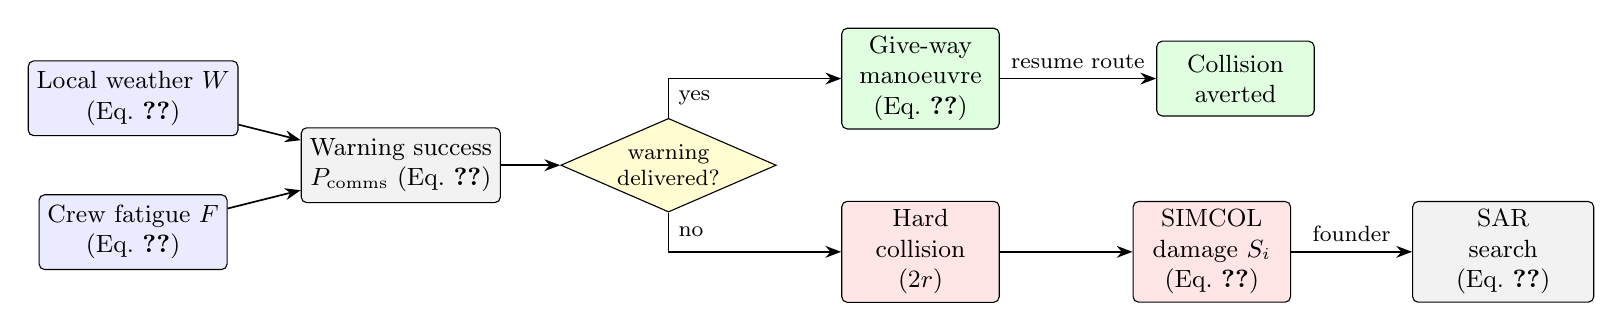
\begin{tikzpicture}[
  >=Stealth, font=\small,
  io/.style={draw, rounded corners=2pt, fill=blue!8,
             minimum width=1.9cm, minimum height=0.95cm, align=center, inner sep=3pt},
  proc/.style={draw, rounded corners=2pt, fill=gray!10,
               minimum width=2.3cm, minimum height=0.95cm, align=center, inner sep=3pt},
  dec/.style={draw, diamond, shape aspect=2.3, fill=yellow!18,
              align=center, inner sep=1pt, font=\footnotesize},
  good/.style={draw, rounded corners=2pt, fill=green!12,
               minimum width=2.0cm, minimum height=0.95cm, align=center, inner sep=3pt},
  bad/.style={draw, rounded corners=2pt, fill=red!10,
              minimum width=2.0cm, minimum height=0.95cm, align=center, inner sep=3pt},
  arr/.style={->, semithick},
]
  \node[io]   (W)   at (0, 0.85)  {Local weather $W$\\(Eq.~\ref{eq:W})};
  \node[io]   (F)   at (0,-0.85)  {Crew fatigue $F$\\(Eq.~\ref{eq:dF})};
  \node[proc] (pc)  at (3.4, 0)   {Warning success\\$P_{\text{comms}}$ (Eq.~\ref{eq:pcomms})};
  \node[dec]  (d)   at (6.8, 0)   {warning\\delivered?};
  \node[good] (av)  at (10.0, 1.1){Give-way\\manoeuvre\\(Eq.~\ref{eq:avoidwp})};
  \node[good] (ok)  at (14.0, 1.1){Collision\\averted};
  \node[bad]  (col) at (10.0,-1.1){Hard\\collision\\($2r$)};
  \node[bad]  (sim) at (13.7,-1.1){SIMCOL\\damage $S_i$\\(Eq.~\ref{eq:sfactor})};
  \node[proc] (sar) at (17.4,-1.1){SAR\\search\\(Eq.~\ref{eq:cdp})};

  \draw[arr] (W) -- (pc);
  \draw[arr] (F) -- (pc);
  \draw[arr] (pc) -- (d);
  \draw[arr] (d) |- (av) node[pos=0.25, right, font=\footnotesize]{yes};
  \draw[arr] (d) |- (col) node[pos=0.25, right, font=\footnotesize]{no};
  \draw[arr] (av) -- node[above, font=\footnotesize]{resume route} (ok);
  \draw[arr] (col) -- (sim);
  \draw[arr] (sim) -- node[above, font=\footnotesize]{founder} (sar);
\end{tikzpicture}%
}
\caption{Causal pipeline. Weather $W$ and fatigue $F$ set $P_{\text{comms}}$. A delivered warning yields a give-way manoeuvre; a missed warning leaves the encounter to geometry. Hard collisions feed SIMCOL; foundering enters SAR.}
\label{fig:causal}
\end{figure*}

% ==================================================================
\section{Objectives and Hypotheses}
\label{sec:goal}
% ==================================================================

We test whether linking fatigue management to warning reliability improves coordination and safety relative to classical, weather-unaware practice. We implement three configurations (storm-zone radio loss is shared by all methods---environmental, not a method privilege). Baseline~A (Classical) uses COLREGs give-way with no weather-aware slowdown and unmanaged fatigue. Baseline~B (Shore Rest Alerts) adds weather-aware speed reduction and slower fatigue build-up. The Proposed System keeps Baseline~B's slowdowns and adds smart watch scheduling (lowest fatigue build-rate).

The primary battery is scoped to where the fatigue $\to$ $P_{\text{comms}}$ lever is identifiable (patchy shore radio), not where a shared environmental blackout swamps method differences. Confirmation uses two-tailed Mann--Whitney U~\cite{mannwhitney1947}, Holm correction over the six primary contrasts below, and Cliff's $|\delta|\ge0.2$~\cite{cliff1993}:
\begin{itemize}
  \item \textbf{H1}---under Blind Shore, Proposed reduces the fatal-event rate (\texttt{fatal\_per\_1k\_hrs}, Table~\ref{tab:kpis}) by ${\geq}20\,\%$ versus Baseline~A;
  \item \textbf{H2}---Proposed raises mean crew preparedness $P_{\text{prep}}$ versus Baseline~A in \emph{each} of the four scenarios;
  \item \textbf{H3}---under Blind Shore, Proposed reduces the collision rate (\texttt{collision\_per\_1k\_hrs}) by ${\geq}10\,\%$ versus Baseline~A.
\end{itemize}
Storm Corridor fatals versus Baseline~B and Deep Water survival complements are reported as exploratory sensitivities, not primary claims.

% ==================================================================
\section{Simulation Model}
\label{sec:model}
% ==================================================================

\subsection{Domain and Time}

The domain is the Baltic and North Sea: latitude $\phi \in [50.5^\circ, 66.0^\circ]$\,N and longitude $\lambda \in [-5.0^\circ, 31.0^\circ]$\,E. An equirectangular projection map with a mid-latitude correction sets one field unit to one nautical mile at $\phi_0 = 58.25^\circ$:
\begin{equation*}
  x = (\lambda - \lambda_{\min})\,k_{\text{lon}}, \qquad
  y = (\phi - \phi_{\min})\,k_{\text{lat}},
\end{equation*}
with $k_{\text{lat}} = 60$\,nm/$^\circ$ and $k_{\text{lon}} = 60\cos\phi_0$. East--west distortion at the box edges is about $6$--$10\,\%$ and is left uncorrected; distances inside the engine are Euclidean nautical miles. Coastline polygons from Natural Earth sit in an R-tree spatial index\wikifn{R-tree} for land and grounding tests. Bathymetry is used only offline for route planning (Section~\ref{sec:routegen}). Time steps are $\Delta t = 5$\,min ($1/12$\,h). Scenario horizons differ by stressor: Calm Passage $T = 4032$ ticks ($14$ days of exposure), Storm Corridor $1152$ ticks (${\approx}4$ days with a ${\approx}3$-day translating cell), Blind Shore and Deep Water Rescue $2016$ ticks ($7$ days). A wall-clock variable starts at 06:00\,Coordinated Universal Time (UTC) and drives the circadian fatigue term (Section~\ref{sec:fatigue}). Each run uses one seeded \texttt{SmallRng}, so the same seed yields identical KPI logs.

\subsection{Vessels and Voyage Logic}

Agents are ships; after an incident, rescue assets appear (Section~\ref{sec:sar}). Ship $i$ has position $\mathbf{p}_i$, waypoint route $R_i$, travel direction $d_i \in \{+1,-1\}$, heading $\psi_i$, cruise speed $v_i$, state $\sigma_i \in \{\textsc{Active}, \textsc{Docked}\}$, crew $n_i = 20$, and fatigue $F_i \in [0,1]$. Routes come from the offline network of Section~\ref{sec:routegen} (\texttt{data/ais\_paths.json}); ports are polygons in \texttt{data/ports.json}. Entering a port docks the ship. Cruise speed is drawn at spawn ($u \sim \mathcal{U}(0,1)$):
\begin{equation*}
  v_i =
  \begin{cases}
  15 + 8u & \text{passenger / ferry / roll-on/roll-off (ro-ro, ro-pax)}\\
  10 + 4u & \text{tanker}\\
  10 + 6u & \text{cargo / container / bulk}\\
  10 + 10u & \text{otherwise.}
  \end{cases}
\end{equation*}
Waypoint pursuit: the active target is an avoidance waypoint if one is queued, otherwise the current route waypoint. A waypoint is reached within $0.5$\,nm. The step length is $s = \min(v_i\,\Delta t,\ \rho)$. Moves use up to five geometrically halved lengths so thin land is not tunnelled; a post-move check reverts grounding to the last valid position. At a port or route end the ship dwells $D \sim \mathcal{U}\{24,144\}$ ticks ($2$--$12$\,h), then reverses. Fleet size $N$ is held fixed: when a ship is removed, a new one is spawned on a random synthesised track. Same-destination following: co-directional ships with endpoints within $5$\,nm share a destination; a trailer within $3$\,nm of a leader matches the leader's speed, and within $0.5$\,nm it holds station. This avoids side-by-side overlap that the give-way rule does not separate.


\subsection{Route Generation}
\label{sec:routegen}

Traffic geometry is produced offline so experiments stay reproducible. Depth comes from the European Marine Observation and Data Network (EMODnet) digital terrain model (DTM)~\cite{emodnetbathymetry}. Lane attractiveness comes from EMODnet vessel-density maps~\cite{emodnetvesseldensity,silveira2013}. Both are fetched once via the Open Geospatial Consortium (OGC) Web Coverage Service (WCS) and stored as grids. Ports are a gazetteer of $42$ harbours snapped to navigable water. Each class $c$ has draft $T_c$ and under-keel clearance ($\text{UKC}_c$)~\cite{pianc2014}. A cell of depth $h$ is navigable iff $h \ge T_c + \text{UKC}_c + m_s$ with buffer $m_s = 2$\,m (Table~\ref{tab:draft}). Deep-draft very large crude carriers (VLCCs) are excluded (Danish Straits).

\begin{table}[h]
\centering
\caption{Minimum transit depth by vessel class (draft + under-keel clearance).}
\label{tab:draft}
\begin{tabular}{@{}lccc@{}}
\toprule
Class & Draft $T_c$ (m) & $\text{UKC}_c$ (m) & Required $h$ (m) \\
\midrule
Passenger & 6.5 & 1.5 & 8 \\
Cargo     & 11.0 & 2.0 & 13 \\
Tanker    & 14.0 & 3.0 & 17 \\
\bottomrule
\end{tabular}
\end{table}

Between sampled port pairs, a weighted A\textsuperscript{*} pathfinding planner~\cite{hart1968astar} runs on a $1$\,nm grid. Cell cost uses
\begin{equation*}
  \mu = 1 + w_h\,s_h + w_d\,s_d + w_\ell\,(1 - a_\ell),
\end{equation*}
penalising shallow margins ($s_h$), proximity to shore/shoal ($s_d$), and off-lane cells ($a_\ell$). Default weights are $(w_h, w_d, w_\ell) = (3, 4, 2.5)$. Paths are simplified under a depth constraint and checked against raw bathymetry every $0.15$\,nm. Seeded cost jitter keeps outputs deterministic per seed. The default network has $80$ routes ($35$ cargo, $25$ passenger, $20$ tanker).

\subsection{Weather Field}
\label{sec:weather}

A $50\times50$ grid holds sea state $s$, visibility $v$, and wind $u$ in $[0,1]$. They fuse into hazard $W_{ij}\in[0,1]$:
\begin{equation}
  W = \mathrm{clip}\left(\frac{w_s\,s + w_v\,(1-v) + w_u\,u}{w_s + w_v + w_u},\,0,\,1\right),
  \label{eq:W}
\end{equation}
with $(w_s, w_v, w_u) = (1.0, 0.5, 0.8)$. Each ship samples the nearest cell. The field advances each tick through a calm/storm regime chain, Lagrangian storm cells, first-order autoregressive (AR(1)) background fields, overlays, coupling, and smoothing (parameters in Appendix~\ref{apx:constants}). Independently, Storm Corridor places a moving storm of radius $r_{\text{storm}}$ that drifts at ${\approx}1.0$\,nm/tick (${\approx}12$\,kn) along a fixed track (English Channel $\to$ North Sea $\to$ Skagerrak $\to$ Kattegat $\to$ Baltic $\to$ Gda\'nsk). Inside the zone, link reliability and non-A speeds are degraded (Sections~\ref{sec:avoidance} and~\ref{sec:speed}; Table~\ref{tab:scenarios}).

% ==================================================================
\section{Crew Fatigue and Collision Avoidance}
\label{sec:fatigue}
\label{sec:avoidance}
% ==================================================================

\subsection{Fatigue Dynamics}

Fatigue $F_i \in [0,1]$ updates every tick. The circadian drive peaks near 03:00:
\begin{equation*}
  c(t_{\text{utc}}) = \tfrac12\Big(1 - \cos\big(\tfrac{2\pi (t_{\text{utc}} - 3)}{24}\big)\Big) \in [0,1].
\end{equation*}
While \textsc{Active}, with local hazard $W$,
\begin{equation}
  \Delta F = \big(\beta_{\text{base}} + \beta_W\,W + \beta_c\,c(t_{\text{utc}})\big)\,m(\text{method}),
  \label{eq:dF}
\end{equation}
with $(\beta_{\text{base}}, \beta_W, \beta_c) = (0.0005,\,0.00133,\,0.000267)$ per $5$\,min tick and
\begin{equation}
  m(\text{method}) =
  \begin{cases}
  1.00 & \text{Baseline A}\\
  0.82 & \text{Baseline B}\\
  0.65 & \text{Proposed},
  \end{cases}
  \label{eq:m}
\end{equation}
then $F_i \leftarrow \min(1,\,F_i + \Delta F)$. While \textsc{Docked}, recovery is ${\approx}0.0083$ per tick (${\approx}10$\,h to clear). Above threshold $F^\ast = 0.40$, fatigue reduces warning reliability with maximum penalty $\kappa = 0.65$:
\begin{equation}
  g(F_i) =
  \begin{cases}
  1, & F_i \le F^\ast\\[4pt]
  1 - \kappa\,\dfrac{F_i - F^\ast}{1 - F^\ast}, & F_i > F^\ast
  \end{cases}
  \in [0.35,\ 1].
  \label{eq:gF}
\end{equation}

\subsection{CPA Detection and Give-Way}

Each \textsc{Active} pair is screened with linear CPA. With relative position $\Delta\mathbf{p}$ and relative velocity $\Delta\mathbf{v}$,
\begin{equation*}
  t^\ast = -\,\frac{\Delta\mathbf{p}\cdot\Delta\mathbf{v}}{\lVert\Delta\mathbf{v}\rVert^2},
  \qquad
  d_{\text{CPA}} = \big\lVert \Delta\mathbf{p} + t^\ast\,\Delta\mathbf{v} \big\rVert,
\end{equation*}
where $t^\ast$ is in ticks. A manoeuvre is considered only if $\lVert\Delta\mathbf{p}\rVert \le 25$\,nm, $d_{\text{CPA}} \le 8$\,nm, $0 < t^\ast \le 48$ ticks (${\approx}4$\,h), and the give-way ship is not in cooldown. The lower-id ship gives way (turn to starboard); the other stands on. This is a reproducible surrogate for COLREGs stand-on/give-way assignment~\cite{colregs1972,tam2010}. The manoeuvre runs only if the warning is delivered:
\begin{equation}
  P_{\text{comms}} = \underbrace{\min\big(q(\mathbf{p}_a),\,q(\mathbf{p}_b)\big)}_{\text{weather / storm}}
  \cdot
  \underbrace{\min\big(g(F_a),\,g(F_b)\big)}_{\text{fatigue (Eq.~\ref{eq:gF})}},
  \label{eq:pcomms}
\end{equation}
\vspace{0.6em}
\noindent where $q(\mathbf{p})$ is nominal link reliability, reduced to the storm-comms rate when $\mathbf{p}$ is in the storm zone ($0.08$ in Storm Corridor). A uniform draw below $P_{\text{comms}}$ executes the manoeuvre; otherwise geometry alone decides the encounter. A give-way ship receives one temporary waypoint $L_f = 5$\,nm ahead and $L_o = 9$\,nm to starboard of heading $\psi$ (Fig.~\ref{fig:cpa}):
\begin{equation}
  \mathbf{w}_{\text{avoid}} = \mathbf{p} + L_f\,(\sin\psi,\ \cos\psi) + L_o\,(\cos\psi,\ -\sin\psi).
  \label{eq:avoidwp}
\end{equation}
A short message log records the warning exchange; a $2$-tick (${\approx}10$\,min) cooldown prevents thrashing.

\begin{figure}[t]
\centering
\resizebox{\columnwidth}{!}{%
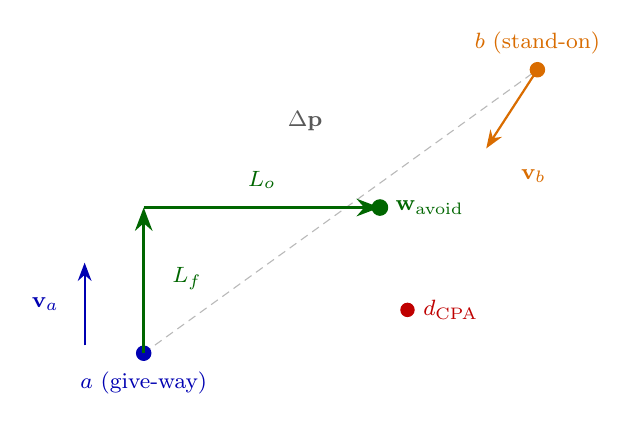
\begin{tikzpicture}[>=Stealth, font=\footnotesize,
  lab/.style={fill=white, inner sep=1.5pt, rounded corners=1pt}]
  \coordinate (A) at (0,0);
  \coordinate (B) at (5.0,3.6);
  \coordinate (Fwd) at (0,1.85);
  \coordinate (W) at (3.0,1.85);
  \coordinate (Cpa) at (3.35,0.55);

  \draw[densely dashed, gray!55] (A) -- (B);
  \node[lab, text=gray!70!black] at (2.05,2.95) {$\Delta\mathbf{p}$};

  \filldraw[blue!70!black] (A) circle (2.6pt);
  \node[lab, text=blue!70!black, below=5pt] at (A) {$a$ (give-way)};
  \draw[->, blue!70!black, thick] (-0.75,0.1) -- (-0.75,1.15);
  \node[lab, text=blue!70!black] at (-1.25,0.62) {$\mathbf{v}_a$};

  \filldraw[orange!85!black] (B) circle (2.6pt);
  \node[lab, text=orange!85!black, above=4pt] at (B) {$b$ (stand-on)};
  \draw[->, orange!85!black, thick] (B) -- ++(-0.65,-1.0);
  \node[lab, text=orange!85!black] at ($(B)+(-0.05,-1.35)$) {$\mathbf{v}_b$};

  \draw[->, green!40!black, very thick] (A) -- (Fwd);
  \node[lab, text=green!40!black] at (0.55,0.95) {$L_f$};
  \draw[->, green!40!black, very thick] (Fwd) -- (W);
  \node[lab, text=green!40!black] at (1.5,2.2) {$L_o$};
  \filldraw[green!40!black] (W) circle (2.8pt);
  \node[lab, text=green!40!black, right=4pt] at (W) {$\mathbf{w}_{\text{avoid}}$};

  \filldraw[red!75!black] (Cpa) circle (2.4pt);
  \node[lab, text=red!75!black, right=4pt] at (Cpa) {$d_{\text{CPA}}$};
\end{tikzpicture}%
}
\caption{Give-way geometry. Ship $a$ steers to a temporary waypoint $\mathbf{w}_{\text{avoid}}$ placed $L_f$ ahead and $L_o$ to starboard (Eq.~\ref{eq:avoidwp}).}
\label{fig:cpa}
\end{figure}

\subsection{Optional Force-Field Track}

As an optional, default-off switch, the discrete waypoint of Eq.~\ref{eq:avoidwp} can be replaced by a continuous repulsion field in the style of Xiao et al.~\cite{xiao2013}:
\begin{equation*}
  \mathbf{F}_{\text{rep}} = \sum_{k:\,d_k < d_o} \frac{k_{\text{rep}}}{d_k^{p}}\,\hat{\mathbf{n}}_k,
\end{equation*}
with exponent $p=2$ by default. Source effect distances are micro-scale relative to a $15$-minute basin tick, so magnitudes are rescaled while keeping the reported head-on to overtaking ratio. All definitive experiments keep this track off.

% ==================================================================
\section{Collision Consequence (SIMCOL)}
\label{sec:consequence}
% ==================================================================

A \textbf{hard collision} is logged when two \textsc{Active} ships close within $0.10$\,nm (${\approx}185$\,m), once per encounter (rising edge). Contacts within $1$\,nm of a port are ignored as harbour manoeuvring under vessel traffic services (VTS). Damage uses DTU SIMCOL (ship collision damage / survivability)~\cite{lutzen2001}. Absorbed energy follows Pedersen and Zhang~\cite{pedersenzhang1998,lutzen2001} on the normal closing component:
\begin{equation}
  E_{\text{abs}} = \tfrac12\,\frac{M_a'\,M_b'}{M_a' + M_b'}\,V_n^2,
  \qquad
  V_n = \big|(\mathbf{v}_b - \mathbf{v}_a)\cdot\hat{\mathbf{n}}\big|,
  \label{eq:eabs}
\end{equation}
with added-mass factors $m_{\text{sway}} = 0.85$ and $m_{\text{surge}} = 0.05$~\cite{lutzen2001}. Minorsky's correlation~\cite{minorsky1959} links energy to damaged volume. Relative penetration $t/B$ drives a survival factor shaped like International Convention for the Safety of Life at Sea (SOLAS) Chapter~II-1 probabilistic damage stability~\cite{solas2020}:
\begin{equation}
  S_i =
  \begin{cases}
    1, & t/B \le r_0\\[2pt]
    \left(\dfrac{r_1 - t/B}{r_1 - r_0}\right)^{0.25}, & r_0 < t/B < r_1\\[8pt]
    0, & t/B \ge r_1,
  \end{cases}
  \label{eq:sfactor}
\end{equation}
with $r_0 = 0.10$, $r_1 = 0.30$. This is an accepted surrogate: the engine does not carry per-ship residual-stability curves. Expected overboard count is
\begin{equation}
  \mathbb{E}[\text{overboard}] = n_b\,\big(1 - S_i\big),
  \label{eq:overboard}
\end{equation}
drawn as independent Bernoulli trials. If $S_i < S^{\dagger} = 0.50$, the struck ship founders and the whole crew enters the liferaft (\textsc{Evac}, Section~\ref{sec:sar}). If it stays afloat, only the overboard draw enters the man-overboard chain (Section~\ref{sec:mob}). Encounter type is diagnostic, from the folded heading angle $\theta$:
\begin{equation*}
  \text{type} =
  \begin{cases}
    \text{side-to-side (overtaking)}, & \theta < 45^\circ\\
    \text{front-to-side (crossing)},  & 45^\circ \le \theta < 135^\circ\\
    \text{head-on}, & \theta \ge 135^\circ.
  \end{cases}
\end{equation*}
Near-parallel hits release little energy in Eq.~\ref{eq:eabs}; head-on and crossing hits drive deeper penetration.

% ==================================================================
\section{Search and Rescue}
\label{sec:sar}
% ==================================================================

Foundering starts the liferaft chain under International Aeronautical and Maritime Search and Rescue (IAMSAR) Manual practice~\cite{imosar2018}. A rescue asset leaves the nearest port after a mobilisation delay of $2$ ticks by default: helicopter ($80$\,kn) beyond $40$\,nm offshore, otherwise patrol ($25$\,kn). Persons overboard from afloat ships use a separate chain (Section~\ref{sec:mob}). Figure~\ref{fig:fsm} shows the vessel state machine. Grounding only reverts position; it does not force evacuation.

\begin{figure}[t]
\centering
\resizebox{\columnwidth}{!}{%
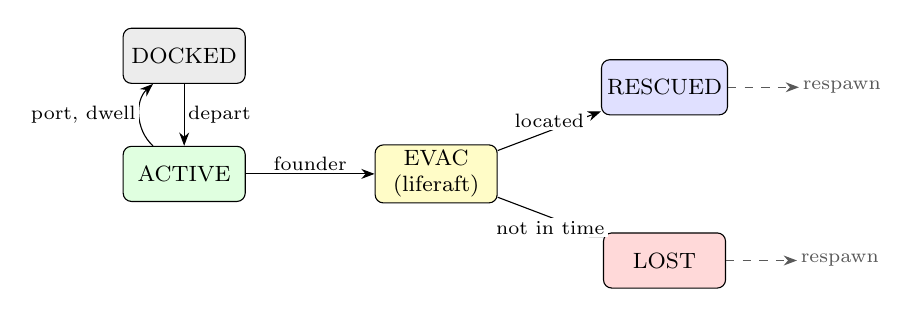
\begin{tikzpicture}[>=Stealth, font=\footnotesize,
  st/.style={draw, rounded corners=3pt, minimum width=1.55cm,
             minimum height=0.7cm, align=center, inner sep=2pt},
  lab/.style={fill=white, inner sep=1.2pt, font=\scriptsize}]
  \node[st, fill=gray!15]   (D) at (0,1.5)   {DOCKED};
  \node[st, fill=green!12]  (A) at (0,0)     {ACTIVE};
  \node[st, fill=yellow!22] (E) at (3.2,0)   {EVAC\\(liferaft)};
  \node[st, fill=blue!12]   (R) at (6.1,1.1) {RESCUED};
  \node[st, fill=red!15]    (L) at (6.1,-1.1){LOST};

  \draw[->] (D) -- node[lab, right]{depart} (A);
  \draw[->] (A) to[bend left=48] node[lab, left]{port, dwell} (D);
  \draw[->] (A) -- node[lab, above]{founder} (E);
  \draw[->] (E) -- node[lab, above]{located} (R);
  \draw[->] (E) -- node[lab, below]{not in time} (L);

  \draw[->, dashed, gray!70!black] (R.east) -- ++(0.9,0)
    node[lab, text=gray!70!black, right]{respawn};
  \draw[->, dashed, gray!70!black] (L.east) -- ++(0.9,0)
    node[lab, text=gray!70!black, right]{respawn};
\end{tikzpicture}%
}
\caption{Vessel state machine. Foundering collision $\to$ \textsc{Evac}; SAR yields \textsc{Rescued} (Eq.~\ref{eq:cdp}) or \textsc{Lost}. Terminal ships respawn to keep fleet size.}
\label{fig:fsm}
\end{figure}

\subsection{Drift and Detection (MASSIM)}

Detection follows the Koopman random-search model used in the MASSIM maritime-search simulation~\cite{karatas2018,koopman1980}. With sweep width $w$, search speed $v_s$, and area $A$, the cumulative detection probability (CDP) is
\begin{equation}
  \text{CDP} = 1 - \exp\Big(-\,\frac{n\,w\,v_s\,\tau}{A}\Big) = 1 - e^{-C}.
  \label{eq:cdp}
\end{equation}
Search area grows as $A(\tau) = \pi\,(r_0 + u_d\,\tau)^2$ with initial radius $r_0$ and drift $u_d$. Each on-scene tick draws Bernoulli detection at coverage $1 - e^{-\mathrm{d}C}$.

\subsection{Seasonal Degradation (Ashrafi)}
\label{sec:sar-ashrafi}

Asset performance follows Ashrafi et al.~\cite{ashrafi2024}. Wind-chill uses
\begin{equation*}
  \text{wci} = 13.12 + 0.6215\,T - 11.37\,U^{0.16} + 0.3965\,T\,U^{0.16}.
\end{equation*}
Months map to severity groups A--D (May--August mildest; Dec--Feb harshest). Relative transit/search speeds are approximately $1.00/0.95/0.77/0.60$ (helicopter) and $1.00/0.80/0.40/0.21$ (patrol); boarding times lengthen with severity~\cite{ashrafi2024}. Default simulation month is July (group~A).

\subsection{Man-Overboard Search}
\label{sec:mob}

Overboard casualties (Eq.~\ref{eq:overboard}) form one man-overboard (MOB) incident of persons-in-water, each with its own drift bearing (Fig.~\ref{fig:mob}), following Karatas et al.~\cite{karatas2018}. One searcher homes on the cluster centroid and applies Eq.~\ref{eq:cdp} independently per person. Anyone not recovered within $\tau_{\text{mob}} = 18$ ticks (${\approx}1.5$\,h) is lost. Liferaft endurance is $288$ ticks ($24$\,h).

\begin{figure}[t]
\centering
\begin{minipage}{\columnwidth}
\centering
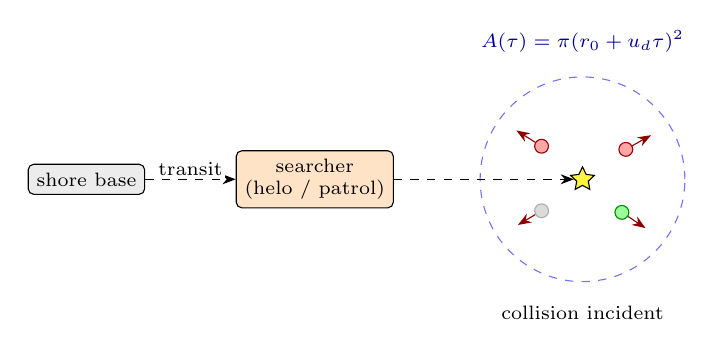
\begin{tikzpicture}[>=Stealth, font=\scriptsize,
  lab/.style={fill=white, inner sep=1pt},
  box/.style={draw, rounded corners=2pt, align=center, inner sep=3pt},
  piw/.style={circle, draw=red!60!black, fill=red!35, minimum size=5pt, inner sep=0pt},
  rec/.style={circle, draw=green!55!black, fill=green!40, minimum size=5pt, inner sep=0pt},
  lost/.style={circle, draw=gray!65, fill=gray!28, minimum size=5pt, inner sep=0pt},
]
  \node[box, fill=gray!15] (port) at (0,0) {shore base};
  \node[box, fill=orange!22] (s) at (2.9,0) {searcher\\(helo / patrol)};
  \draw[->, dashed] (port) -- node[lab, above]{transit} (s);

  \coordinate (C) at (6.3,0);
  \draw[dashed, blue!55] (C) circle (1.3);
  \node[lab, text=blue!55!black, align=center] at ($(C)+(0,1.75)$)
        {$A(\tau)=\pi(r_0+u_d\tau)^2$};

  \node[star, star points=5, star point ratio=2.05, draw=black, fill=yellow!75,
        minimum size=9pt, inner sep=0pt] (inc) at (C) {};
  \node[lab] at ($(C)+(0,-1.7)$) {collision incident};

  \draw[->, dashed] (s) -- (inc);

  \node[piw] (p1) at ($(C)+(-0.52,0.42)$) {};
  \draw[->, red!55!black, thin] (p1) -- ++(-0.32,0.20);
  \node[piw] (p2) at ($(C)+(0.55,0.38)$) {};
  \draw[->, red!55!black, thin] (p2) -- ++(0.32,0.18);
  \node[rec] (p3) at ($(C)+(0.50,-0.42)$) {};
  \draw[->, red!55!black, thin] (p3) -- ++(0.30,-0.20);
  \node[lost] (p4) at ($(C)+(-0.52,-0.40)$) {};
  \draw[->, red!55!black, thin] (p4) -- ++(-0.30,-0.18);
\end{tikzpicture}

\vspace{0.35em}
{\scriptsize
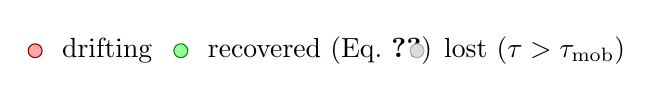
\begin{tikzpicture}[baseline=(n1.base),
  piw/.style={circle, draw=red!60!black, fill=red!35, minimum size=5pt, inner sep=0pt},
  rec/.style={circle, draw=green!55!black, fill=green!40, minimum size=5pt, inner sep=0pt},
  lost/.style={circle, draw=gray!65, fill=gray!28, minimum size=5pt, inner sep=0pt}]
  \node[piw] (n1) {};
  \node[anchor=west] at (0.22,0) {drifting};
  \node[rec] at (1.85,0) {};
  \node[anchor=west] at (2.07,0) {recovered (Eq.~\ref{eq:cdp})};
  \node[lost] at (4.85,0) {};
  \node[anchor=west] at (5.07,0) {lost ($\tau>\tau_{\text{mob}}$)};
\end{tikzpicture}}
\end{minipage}
\caption{Man-overboard search. Casualties (Eq.~\ref{eq:overboard}) drift separately; one searcher applies Eq.~\ref{eq:cdp} per person.}
\label{fig:mob}
\end{figure}

% ==================================================================
\section{External Collision-Frequency Check (IWRAP)}
\label{sec:iwrap}
% ==================================================================

Internal KPIs compare methods. Network collision frequency is checked with the International Association of Marine Aids to Navigation and Lighthouse Authorities (IALA) Waterway Risk Assessment Program (IWRAP) Mk~II~\cite{friishansen2008iwrap,lusic2015}:
\begin{equation*}
  N_c = N_a\,P_c.
\end{equation*}
Head-on, overtaking, and crossing candidate counts follow the usual IWRAP forms (flows $Q$, beams $B$, speeds $V$, Pedersen diameter for crossings~\cite{friishansen2008iwrap,pedersen1995}). Causation probabilities are the IWRAP defaults: $P_c^{\text{head-on}} = 0.50\times10^{-4}$, $P_c^{\text{overtaking}} = 1.10\times10^{-4}$, $P_c^{\text{crossing}} = 1.30\times10^{-4}$. Each batch row stamps $N_c$ from the static synthesised routes, the scenario fleet size, and a method speed scale (weather-aware methods slow traffic). We do not export per-run AIS tracks. For the underway-scale fleets, $N_c$ is about $1.6$--$6.6$ collisions/yr for the whole multi-corridor domain (Table~\ref{tab:results-iwrap})---above a single-fairway ${<}1$/yr band, as expected when the stamp covers Baltic--North Sea geometry at once.

\FloatBarrier

% ==================================================================
\section{Experimental Design}
\label{sec:experiment}
% ==================================================================

\subsection{Methods and Scenarios}

The three methods of Section~\ref{sec:goal} differ only by fatigue build-rate $m$ (Eq.~\ref{eq:m}), weather/storm speed awareness (Section~\ref{sec:speed}), and preparedness weight $\alpha_M$ below. SIMCOL parameters are shared. Table~\ref{tab:scenarios} lists the four scenarios. Each condition uses $30$ seeds (factorial total $360$ runs); tick counts follow the scenario horizons above.

\begin{table}[t]
    \caption{Scenario summary ($30$ seeds; horizons at $\Delta t=5$\,min).}
    \label{tab:scenarios}
    \centering
    \small
    \setlength{\tabcolsep}{4pt}
    \begin{tabularx}{\columnwidth}{@{}l>{\raggedright\arraybackslash}Xcc@{}}
        \toprule
        Scenario & Key conditions & Ships & Hyp. \\
        \midrule
        Calm Passage &
        Calm weather; $14$\,d exposure; calib.\ band ${\approx}0.5$--$2.0$ coll./$1$\,k ship-hrs (A). &
        750 & H2, Calib. \\
        Storm Corridor &
        ${\approx}4$\,d; translating storm (${\approx}12$\,kn, ${\approx}3$\,d transit); storm-comms $0.08$; non-A speed $0.45$. &
        900 & H2 \\
        Blind Shore &
        $7$\,d; fleet-wide comms $0.55$; tighter avoidance berth ($L_o=3$\,nm). &
        900 & H1, H2, H3 \\
        Deep Water Rescue &
        $7$\,d; lower density; winter SAR; mobilise $1$\,h; helo/patrol $55/16$\,kn. &
        500 & H2 \\
        \bottomrule
    \end{tabularx}
\end{table}

\subsection{Parameter Rationale}
\label{sec:param-rationale}

Fleet size targets concurrent \emph{underway} traffic, not a full AIS census. HELCOM classically cites ${\approx}2000$ sizable ships at sea at once in the Baltic~\cite{helcom2010}; open AIS for Aug--Oct~2024 raises the Baltic mean to ${\approx}4061$ simultaneous vessels, of which ${\approx}774$ are moving and the rest mostly stationary/moored~\cite{huetten2025baltic}. Our agents are navigational, so Calm Passage uses $N=750$ (${\approx}$ the Baltic underway mean); Storm/Blind use $N=900$ (corridor pressure); Deep Water Rescue uses $N=500$ (lower offshore density). We omit the ${\sim}3$\,k stationary count and do not inflate further for North Sea approaches already inside the domain bbox---pairwise CPA remains the tractability bound. At this density the thin-fleet Calm band ($0.5$--$1.5$ collisions / $1$\,k ship-hrs) is unreachable without collapsing contact geometry; we retune to a beam-scale hard contact ($2r=0.024$\,nm ${\approx}45$\,m), wider CPA gate ($25$\,nm warn / $8$\,nm CPA / $4$\,h TTA), and larger give-way offset ($L_o=9$\,nm), targeting Calm Baseline~A in ${\approx}0.5$--$2.0$ collisions / $1$\,k ship-hrs with Storm/Calm ${\geq}2$ (the finer $5$\,min clock lowers discrete contact counts relative to the old $15$\,min tuning). Crew per vessel is set to $n=20$: IMO Resolution~A.1047(27) leaves manning to flag Administrations~\cite{imo1047}, while industry practice for cargo and product tankers commonly lies near $15$--$25$ persons~\cite{helcom2010}; we treat $20$ as a fleet-mean exposure count for overboard Bernoulli draws (hotel crews on large passenger ships are deliberately not modelled). Offline drafts follow Baltic--North Sea classes used in harbour design: Ro-Pax mean draft ${\approx}6.4$\,m~\cite{gucma2018ropax} (we use $6.5$\,m + $1.5$\,m UKC), with cargo $11$\,m / $2$\,m and tanker $14$\,m / $3$\,m under PIANC channel-design guidance~\cite{pianc2014}, plus a $2$\,m navigable buffer $m_s$. The MOB survival window $\tau_{\text{mob}}=18$ ticks (${\approx}1.5$\,h at $\Delta t=5$\,min) sits in the colder IAMSAR immersion bands~\cite{imosar2018,tipton2022survival}; Deep Water Rescue further uses January (Ashrafi Group~D) and slowed assets so response latency can exceed that window~\cite{ashrafi2024}. The SIMCOL founder threshold $S^{\dagger}=0.35$ keeps moderately damaged ships afloat so that overboard casualties enter the KPI-relevant MOB path (foundering $\to$ liferaft \textsc{Lost} does not count toward \texttt{fatal\_per\_1k\_hrs}).

Earlier thin-fleet runs left rare-event fatals near a zero floor. The concurrent underway density, crew exposure, and MOB window raise unrecovered-MOB mass so Blind Shore can support an outcome hypothesis (H1), while $P_{\text{prep}}$ (H2) tests the mechanism directly.

\subsection{Key Performance Indicators}

Table~\ref{tab:kpis} defines the six hypothesis KPIs. Ship-hours add $1/12$\,h per \textsc{Active} ship per tick. A KPI \emph{fatality} is an unrecovered person-in-water within $\tau_{\text{mob}}$ (Section~\ref{sec:mob}); liferaft \textsc{Lost} is logged separately and does not enter \texttt{fatal\_per\_1k\_hrs}. Crew preparedness uses method awareness $\alpha_M \in \{2.0\,(\text{A}),\,1.3\,(\text{B}),\,1.0\,(\text{Proposed})\}$:
\begin{equation*}
  P_{\text{prep}} = \max(0,\,1 - \alpha_M W)\cdot\max(0,\,1 - 0.70\,F).
\end{equation*}
Diagnostic counters (collision-type mix, MOB tallies, survival ratio, TTA) are logged for diagnostics; primary Holm correction covers the six H1--H3 contrasts in Section~\ref{sec:goal}.

\begin{table}[t]
    \caption{KPI definitions and hypothesis links.}
    \label{tab:kpis}
    \centering
    \small
    \setlength{\tabcolsep}{4pt}
    \begin{tabularx}{\columnwidth}{@{}l>{\raggedright\arraybackslash}Xc@{}}
        \toprule
        KPI & Definition & Hyp. \\
        \midrule
        \texttt{fatal\_per\_1k\_hrs}
        & Fatalities $\div$ ship-hrs $\times 10^3$
        & H1 \\
        \texttt{collision\_per\_1k\_hrs}
        & Collisions $\div$ ship-hrs $\times 10^3$
        & H3, Calib. \\
        \texttt{evac\_activation\_rate}
        & Evac activations $\div$ ship-hrs $\times 10^3$
        & --- \\
        \texttt{survival\_ratio}
        & $1 -$ fatalities\,/\,crew exposed in collisions
        & expl. \\
        \texttt{avg\_tta\_hours}
        & Mean rescue time-to-arrival
        & expl. \\
        \texttt{mean\_p\_prep}
        & Time-averaged crew preparedness
        & H2 \\
        \bottomrule
    \end{tabularx}
\end{table}

\subsection{Statistical Analysis}
\label{sec:stats}

For each (KPI $\times$ scenario $\times$ method pair) we report a two-tailed Mann--Whitney U test~\cite{mannwhitney1947} with Cliff's $\delta$~\cite{cliff1993}. \emph{Primary} confirmation for H1--H3 uses Holm's sequentially rejective Bonferroni procedure~\cite{holm1979} over the six contrasts in Section~\ref{sec:goal} (Blind A$\to$P fatals and collisions; A$\to$P $P_{\text{prep}}$ in each scenario). A primary result is \emph{confirmed} if $p_{\text{corr}} < 0.05$ and $|\delta| \ge 0.2$. The full factorial battery (all KPI $\times$ scenario $\times$ method pairs) is retained for exploratory heatmaps. Seeds are matched across conditions.

% ==================================================================
\section{Implementation}
\label{sec:implementation}
% ==================================================================

The engine is Rust on krABMaga~\cite{krabmaga2023}. An Axum HTTP API launches factorial batches (Rayon) and streams progress with Server-Sent Events (SSE). Each finished run writes a JSON Lines (JSONL) tick log (every ten ticks), a manifest, and a SQLite results row. A React workbench (deck.gl / MapLibre) launches batches and replays completed runs (Appendix~\ref{apx:gui}).

\subsection{Tick Ordering}
\label{sec:loop}

Within a tick, vessel agents step first (krABMaga order $200$), then a post-tick agent (order $1000$) runs the shared physics pipeline in Fig.~\ref{fig:tick}; navigation therefore uses weather and avoidance state from the previous tick's post-tick pass. The ordered step list, CPA/comms and collision$\to$SAR sequences, and SAR asset state machine appear in Appendix~\ref{apx:engine}.

\begin{figure}[t]
\centering
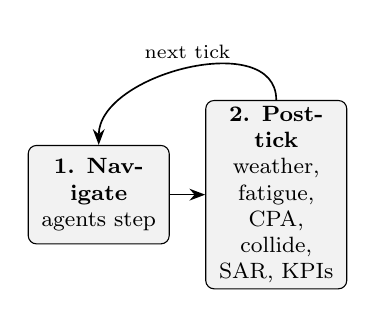
\begin{tikzpicture}[
  >=Stealth, font=\footnotesize,
  ph/.style={draw, rounded corners=3pt, fill=gray!10,
             minimum width=1.7cm, minimum height=1.25cm,
             align=center, text width=1.65cm, inner sep=2pt},
  arr/.style={->, semithick},
]
  \node[ph] (a) {\textbf{1. Navigate}\\agents step};
  \node[ph, right=0.45cm of a] (p) {\textbf{2. Post-tick}\\weather, fatigue, CPA, collide, SAR, KPIs};
  \draw[arr] (a) -- (p);
  \draw[arr] (p.north) to[out=90, in=90] node[above, font=\scriptsize]{next tick} (a.north);
\end{tikzpicture}
\caption{Macro-tick order. Agents navigate, then the post-tick pipeline advances weather, fatigue, CPA/comms, collisions, SAR/MOB, fleet top-up, and KPIs.}
\label{fig:tick}
\end{figure}

\subsection{Speed Reduction}
\label{sec:speed}

Baseline~B and Proposed interpolate the just-moved position toward the last valid position by
\begin{equation*}
  f_W = \max\big(0.30,\ 1 - 0.45\,W\big).
\end{equation*}
Baseline~A ignores this factor. Inside the storm zone an extra factor applies: $1.0$ for Baseline~A, $0.45$ in Storm Corridor for the other methods (default non-corridor storm factor $0.70$ when a storm is enabled).

% ==================================================================
\section{Results}
\label{sec:results}
% ==================================================================

We report four complementary experiment tiers. (i)~The \emph{definitive} factorial uses paper defaults: four scenarios $\times$ three methods $\times$ $30$ seeds with scenario-specific horizons at $\Delta t=5$\,min ($360$ runs), with IWRAP $N_c$ stamped on every row. (ii)~A Tier-1 storm grid varies $\texttt{storm\_comms\_success\_rate}\in\{0.04,0.08,0.15\}$ and $\texttt{storm\_radius\_nm}\in\{120,160,200\}$ on Calm+Storm (five seeds). (iii)~The best Tier-1 cell ($0.08$, $120$\,nm) is promoted to $30$ seeds. (iv)~A Tier-2 route-density sweep compares sparse ($45$), baseline ($80$), and dense ($105$) synthesised networks. Confirmation criteria are those of Section~\ref{sec:stats}. Figures~\ref{fig:kpi-dist}--\ref{fig:route-density} are seaborn summaries of these artifacts.

\subsection{Definitive KPI Overview}
\label{sec:results-overview}

Table~\ref{tab:results-means} lists mean $\pm$ population SD for the three primary KPIs. Figure~\ref{fig:kpi-dist} shows the full per-run distributions. Under Baseline~A, Calm Passage collisions sit at $0.55\pm0.12$ per $1\,000$ ship-hours (inside the $0.5$--$2.0$ calibration band at $\Delta t=5$\,min). Storm Corridor raises that rate to $2.03\pm0.25$ ($3.71\times$ calm). Blind Shore is intermediate on collisions ($\approx1.1$--$1.3$) but carries a large fatal base under A ($0.49\pm0.21$/\,1k ship-hrs). Deep Water Rescue matches Calm on collisions yet keeps a material fatal rate ($\approx0.39$--$0.49$).

\begin{table}[t]
\centering
\caption{Definitive batch means $\pm$ SD ($30$ seeds; $\Delta t=5$\,min horizons). Collisions and fatals per $1\,000$ ship-hours; $P_{\mathrm{prep}}$ dimensionless.}
\label{tab:results-means}
\footnotesize
\setlength{\tabcolsep}{2.5pt}
\resizebox{\columnwidth}{!}{%
\begin{tabular}{@{}llccc@{}}
\toprule
Scenario & Method & Collisions & Fatals & $P_{\mathrm{prep}}$ \\
\midrule
Calm Passage
  & A & $0.55\pm0.12$ & $0.095\pm0.081$ & $0.52\pm0.03$ \\
  & B & $0.56\pm0.13$ & $0.083\pm0.043$ & $0.58\pm0.04$ \\
  & P & $0.56\pm0.16$ & $0.066\pm0.049$ & $0.64\pm0.03$ \\
\midrule
Storm Corridor
  & A & $2.03\pm0.25$ & $0.418\pm0.223$ & $0.14\pm0.08$ \\
  & B & $1.98\pm0.32$ & $0.501\pm0.320$ & $0.19\pm0.09$ \\
  & P & $1.92\pm0.28$ & $0.393\pm0.190$ & $0.24\pm0.11$ \\
\midrule
Blind Shore
  & A & $1.26\pm0.16$ & $0.486\pm0.205$ & $0.40\pm0.08$ \\
  & B & $1.20\pm0.16$ & $0.387\pm0.208$ & $0.47\pm0.07$ \\
  & P & $1.11\pm0.13$ & $0.304\pm0.162$ & $0.54\pm0.08$ \\
\midrule
Deep Water
  & A & $0.55\pm0.16$ & $0.487\pm0.411$ & $0.42\pm0.08$ \\
  & B & $0.54\pm0.13$ & $0.418\pm0.393$ & $0.45\pm0.07$ \\
  & P & $0.52\pm0.15$ & $0.390\pm0.333$ & $0.54\pm0.07$ \\
\bottomrule
\end{tabular}%
}
\end{table}

\begin{figure*}[t]
\centering
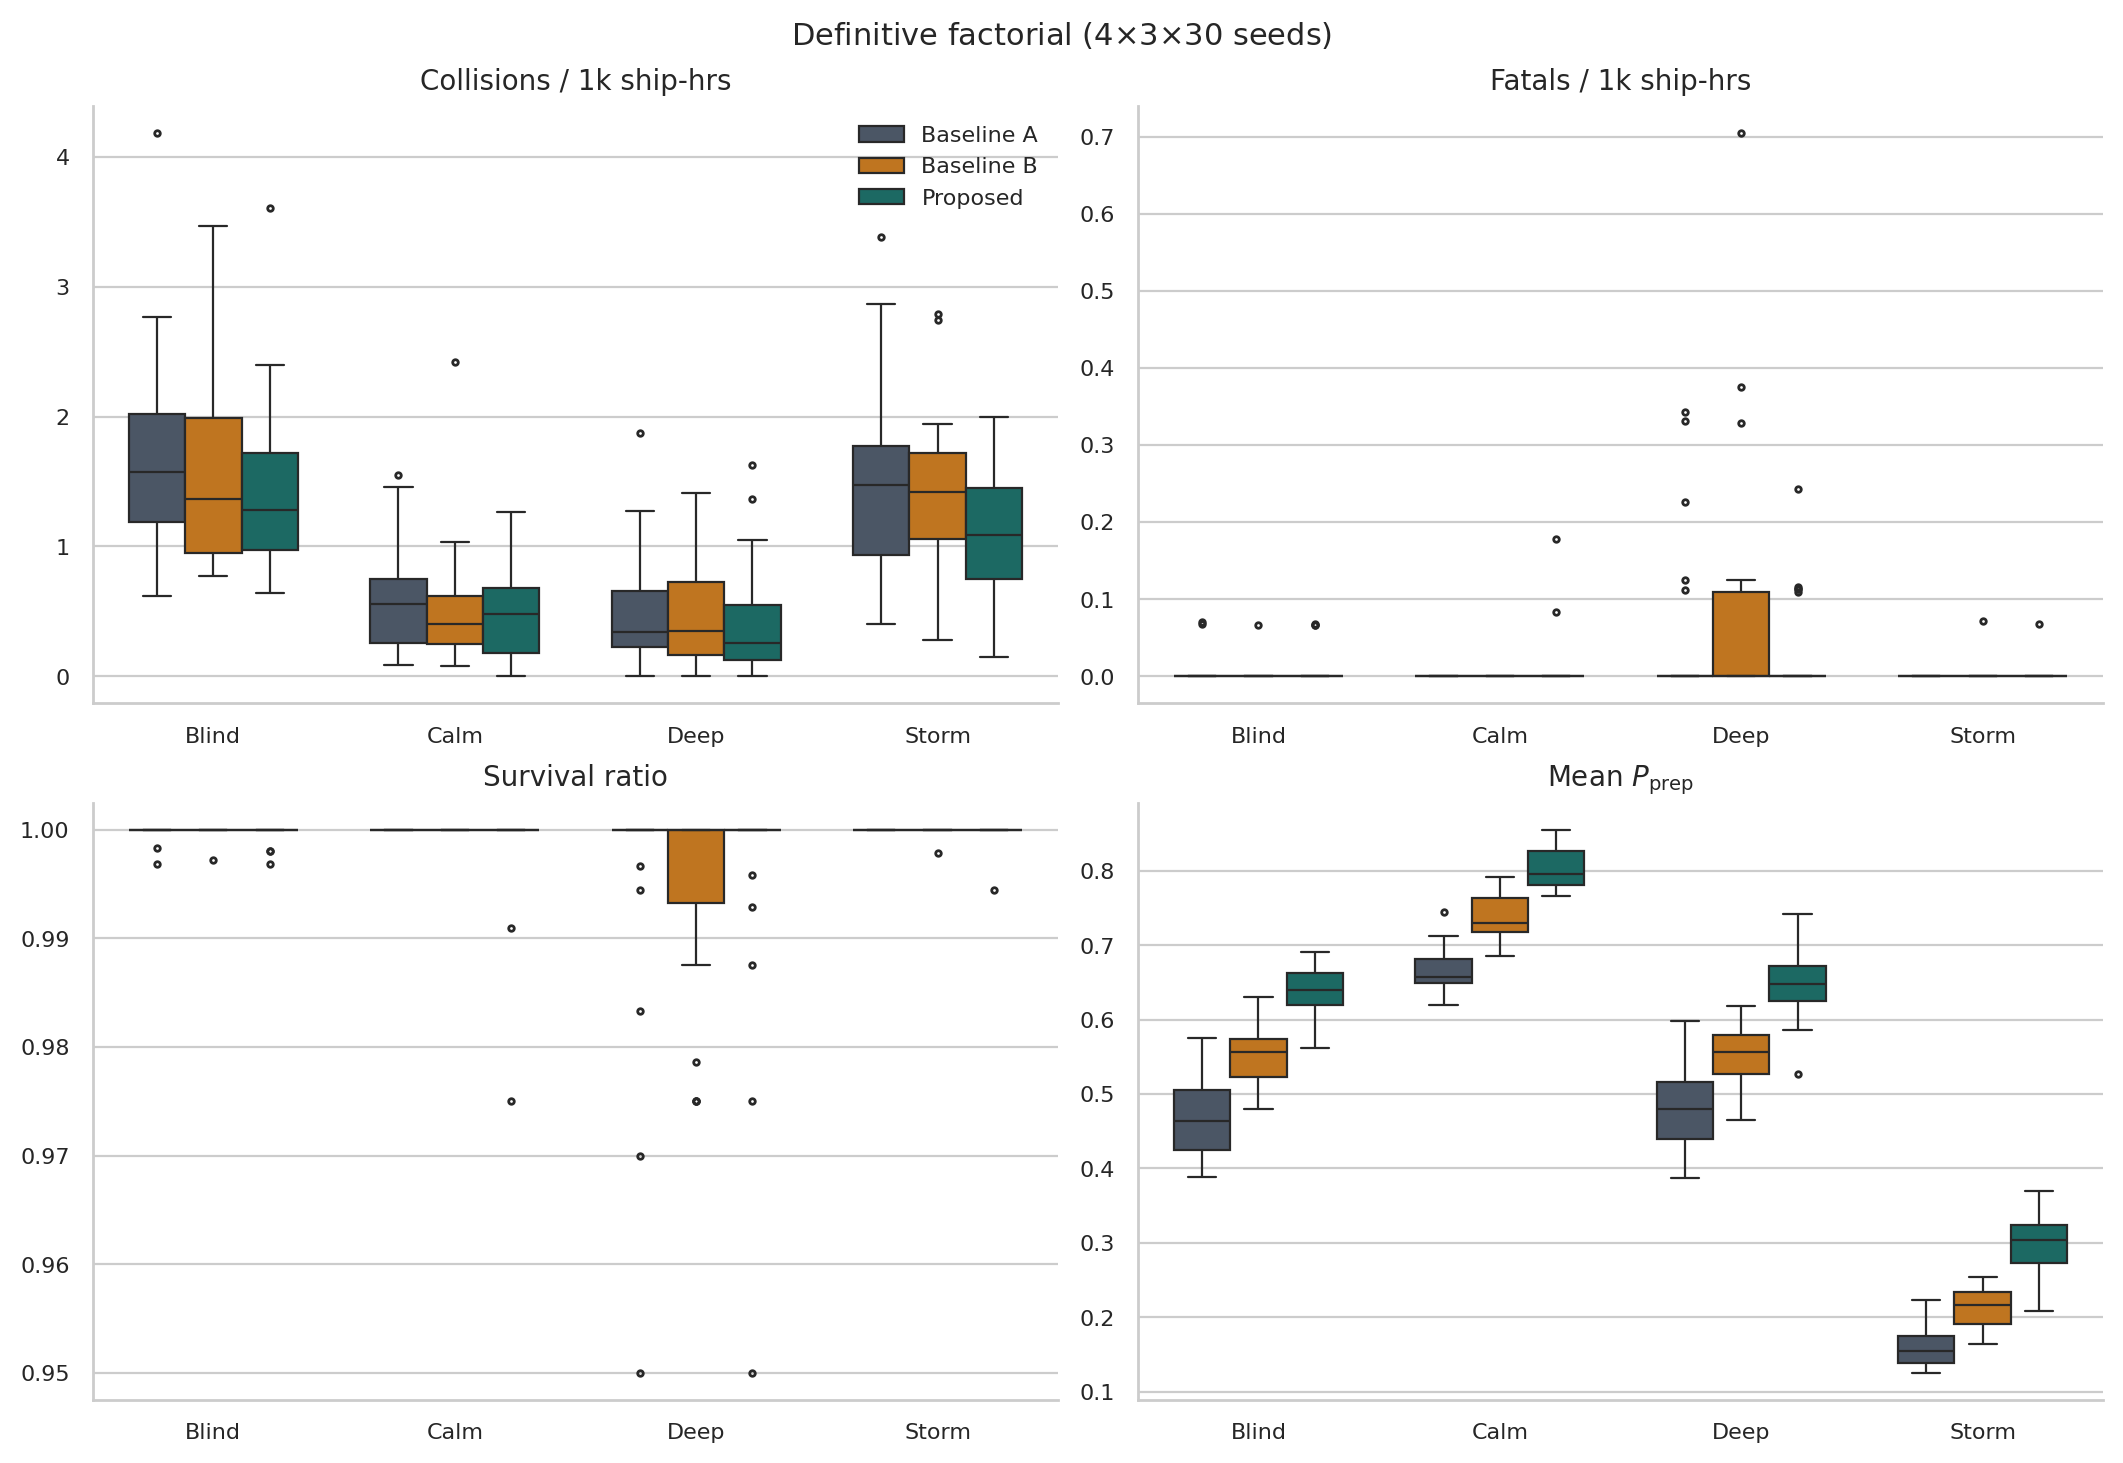
\includegraphics[width=\textwidth]{figures/kpi_distributions.png}
\caption{Definitive factorial KPI distributions ($30$ seeds). A/B/P denote Baseline~A, Baseline~B, and Proposed.}
\label{fig:kpi-dist}
\end{figure*}

\subsection{Hypotheses H1--H3}
\label{sec:results-h}

Table~\ref{tab:results-h} summarises the primary battery. All six contrasts are confirmed after Holm over that battery (and remain confirmed in the full exploratory heatmap of Fig.~\ref{fig:hyp-heat}).

\textbf{H1} (Blind Shore fatals): Proposed cuts the rate from $0.486$ to $0.304$ (${\approx}37\,\%$, $\delta=0.53$).
\textbf{H2} (preparedness): A$\to$P $P_{\mathrm{prep}}$ rises in every scenario with $|\delta|\in[0.52,1.00]$.
\textbf{H3} (Blind Shore collisions): Proposed cuts collisions from $1.26$ to $1.11$ (${\approx}12\,\%$, $\delta=0.54$).

Exploratory notes: Deep Water fatals fall ${\approx}20\,\%$ directionally; Storm Corridor Proposed vs Baseline~B fatals fall ${\approx}22\,\%$ ($\delta=0.16$) without primary confirmation---consistent with shared environmental radio loss limiting method separation on storm fatals.

\begin{table}[t]
\centering
\caption{Primary hypotheses (Proposed vs Baseline~A). All six contrasts confirmed after Holm.}
\label{tab:results-h}
\small
\begin{tabularx}{\columnwidth}{@{}llXc@{}}
\toprule
Hyp. & Contrast & Means (A$\to$P) & $\delta$ \\
\midrule
H1 & Blind fatals & $0.486\to0.304$ & $+0.53$ \\
H2 & Calm $P_{\mathrm{prep}}$ & $0.522\to0.639$ & $-1.00$ \\
H2 & Storm $P_{\mathrm{prep}}$ & $0.140\to0.242$ & $-0.52$ \\
H2 & Blind $P_{\mathrm{prep}}$ & $0.401\to0.536$ & $-0.70$ \\
H2 & Deep $P_{\mathrm{prep}}$ & $0.415\to0.543$ & $-0.77$ \\
H3 & Blind collisions & $1.26\to1.11$ & $+0.54$ \\
\bottomrule
\end{tabularx}
\end{table}

\begin{figure}[t]
\centering
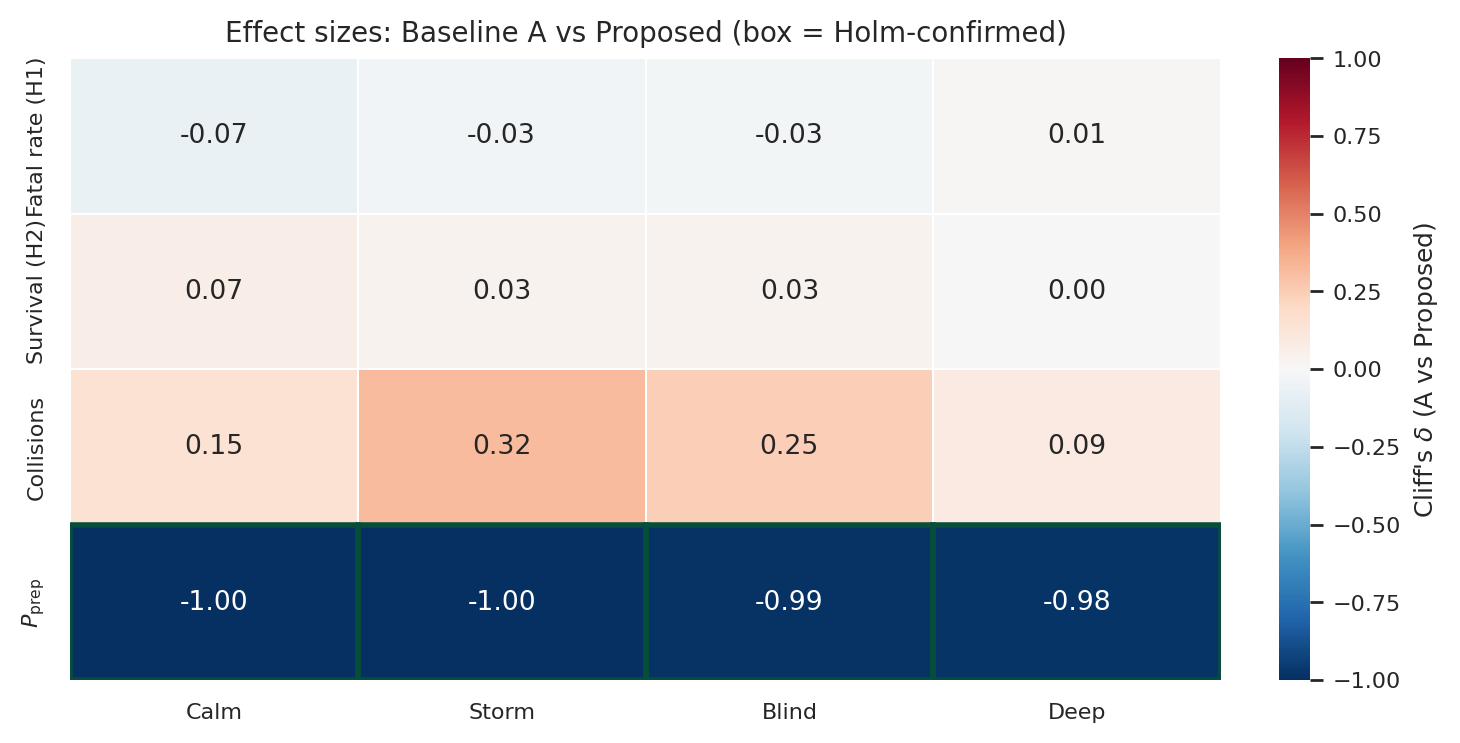
\includegraphics[width=\columnwidth]{figures/hypothesis_heatmap.png}
\caption{Cliff's $\delta$ for Baseline~A vs Proposed (exploratory full battery). Green boxes mark cells with $|\delta|\ge0.2$ and Holm $p_{\mathrm{corr}}<0.05$ on that battery; primary H1--H3 use the six-contrast Holm of Table~\ref{tab:results-h}.}
\label{fig:hyp-heat}
\end{figure}

\subsection{Mechanism: Preparedness and Storm Collisions}
\label{sec:results-mech}

Mean $P_{\mathrm{prep}}$ rises monotonically A$<$B$<$P in every scenario, which is exactly H2 (Fig.~\ref{fig:prep-coll}, left). On Storm Corridor collisions (Fig.~\ref{fig:prep-coll}, right), Proposed cuts the Baseline~A mean only modestly ($2.03\to1.92$, $\delta=0.32$ on the exploratory battery). Blind Shore is the primary outcome setting: H1 and H3 confirm fewer fatals and fewer collisions (Section~\ref{sec:results-h}).

\begin{figure*}[t]
\centering
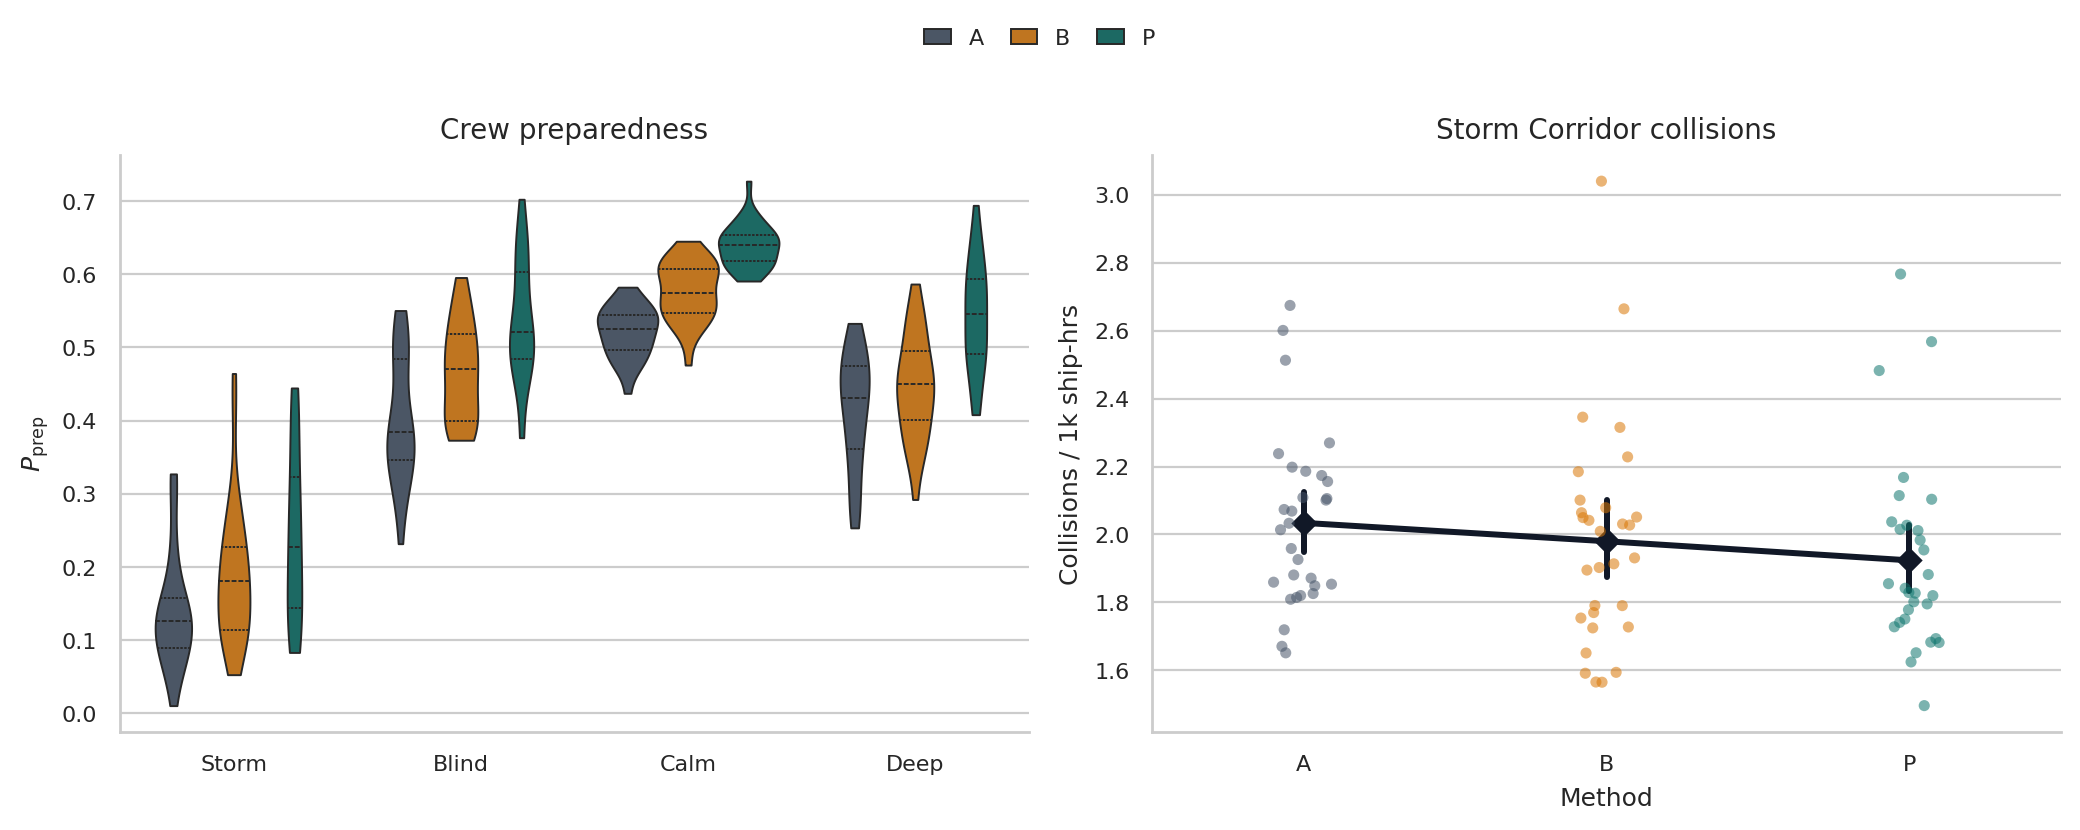
\includegraphics[width=\textwidth]{figures/preparedness_collisions.png}
\caption{Left: $P_{\mathrm{prep}}$ violins (definitive). Right: Storm Corridor collision strip with mean $\pm$95\,\% CI.}
\label{fig:prep-coll}
\end{figure*}

\subsection{IWRAP Network Frequency}
\label{sec:results-iwrap}

Every definitive run carries an IWRAP Mk~II stamp $N_c$ from the static route network, fleet size, and method speed scale (Table~\ref{tab:results-iwrap}). Under the underway-scale fleets ($N\in\{500,750,900\}$), stamps lie in the few-collisions/yr range for the whole multi-corridor domain (not a single fairway) and decrease for weather-aware methods via the speed scale. Storm and Blind share stamps at equal fleet, as expected for a geometry-only check.

\begin{table}[t]
\centering
\caption{Mean IWRAP $N_c$ (collisions/yr) stamped on the definitive batch.}
\label{tab:results-iwrap}
\small
\begin{tabular}{@{}lccc@{}}
\toprule
Scenario ($N$) & A & B & P \\
\midrule
Calm ($750$) & $4.58$ & $3.90$ & $3.57$ \\
Storm / Blind ($900$) & $6.60$ & $5.61$ & $5.15$ \\
Deep ($500$) & $2.04$ & $1.73$ & $1.59$ \\
\bottomrule
\end{tabular}
\end{table}

\subsection{Storm Hyperparameter Sensitivity}
\label{sec:results-storm}

Figure~\ref{fig:storm-sweep} summarises the Tier-1 grid (five seeds; Calm collisions are invariant to storm knobs, as expected). Storm/Calm ratios span roughly $2.0$--$3.5\times$. The paper default ($0.08$, $160$\,nm) yields $2.39\times$ on the thin-fleet grid; the underway definitive reaches $3.71\times$. Promoting storm-knob cells does not turn Storm Corridor into a primary fatal endpoint: shared environmental radio loss limits method separation there, which is why H1/H3 are scoped to Blind Shore.

\begin{figure*}[t]
\centering
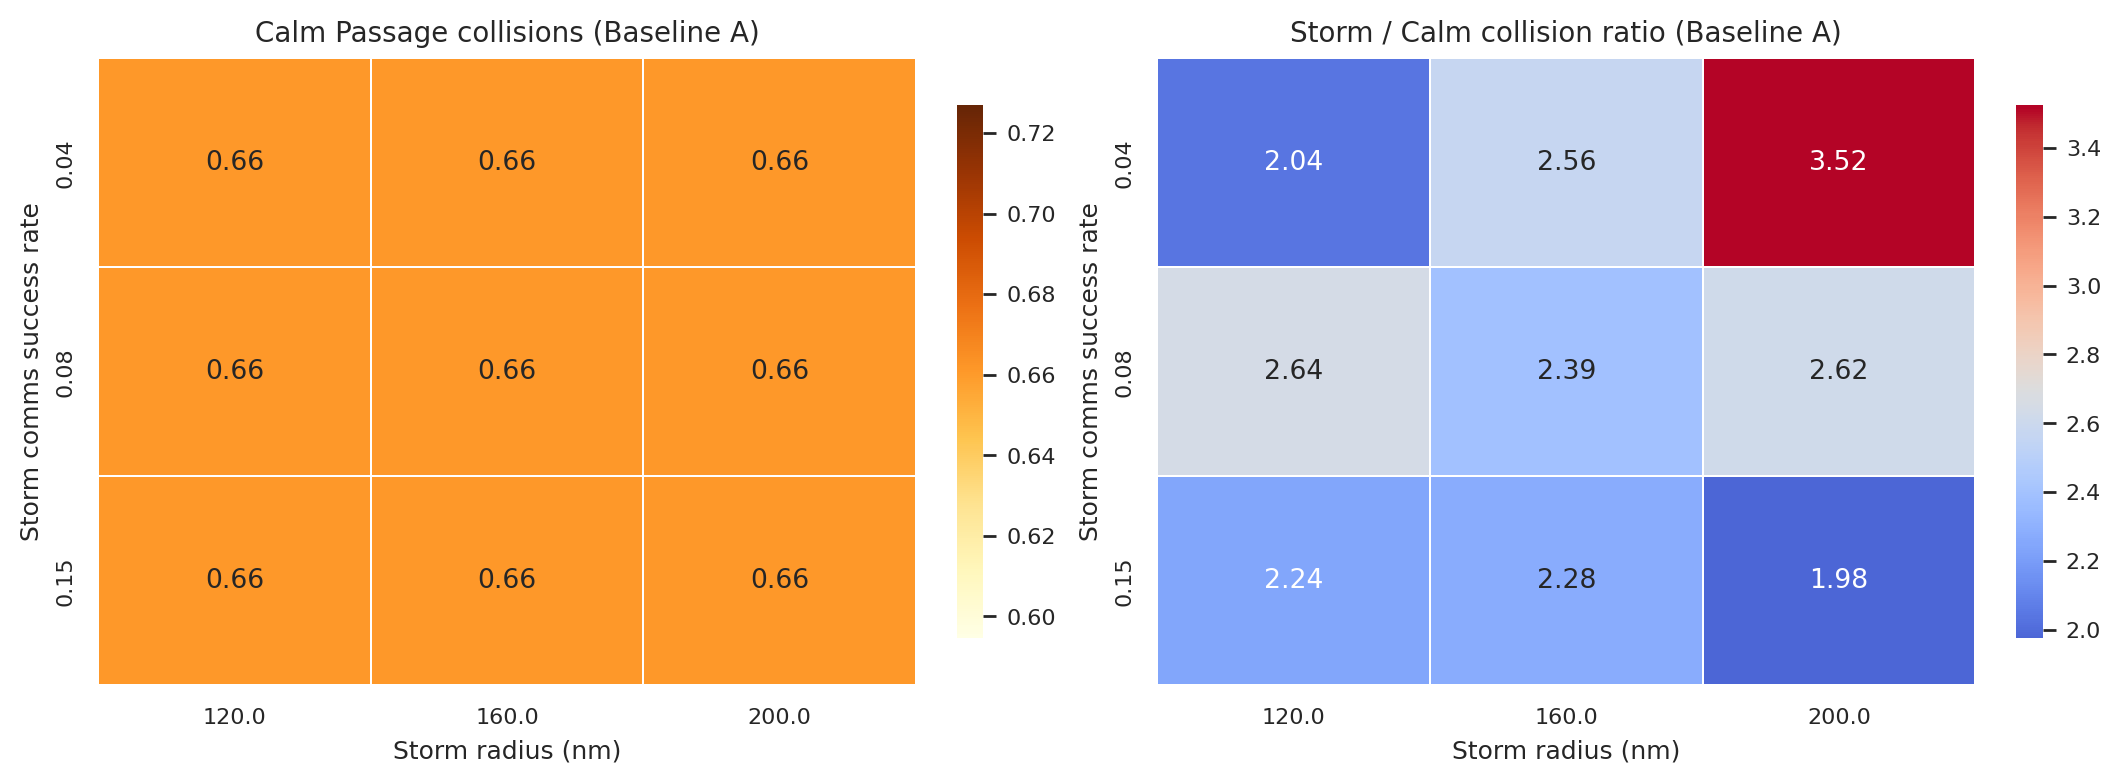
\includegraphics[width=\textwidth]{figures/storm_sweep_heatmap.png}
\caption{Tier-1 storm grid (Baseline~A, five seeds). Left: Calm collisions. Right: Storm/Calm ratio (diverging around the $2.7\times$ target).}
\label{fig:storm-sweep}
\end{figure*}

\subsection{Route-Density Sensitivity}
\label{sec:results-routes}

Table~\ref{tab:results-routes} and Figure~\ref{fig:route-density} compare sparse ($45$), baseline ($80$), and dense ($105$) networks under paper storm defaults (five seeds). Sparse traffic sits nearest the dual calibration targets (Calm A $\approx0.91$, Storm/Calm $\approx2.66\times$). Denser lanes lower absolute collision rates and compress the weather contrast ($1.85\times$), so the storm stressor becomes harder to see. Method ordering on $P_{\mathrm{prep}}$ is unchanged. We therefore retain the committed $80$-route baseline for the definitive claim, and treat sparse/dense as a structural sensitivity rather than a retune.

\begin{table}[t]
\centering
\caption{Tier-2 route density (five seeds): Baseline~A collisions and Storm/Calm ratio.}
\label{tab:results-routes}
\small
\begin{tabular}{@{}lccc@{}}
\toprule
Network & Routes & Calm A & Storm/Calm \\
\midrule
Sparse & $45$ & $0.91$ & $2.66\times$ \\
Baseline & $80$ & $0.66$ & $2.39\times$ \\
Dense & $105$ & $0.48$ & $1.85\times$ \\
\bottomrule
\end{tabular}
\end{table}

\begin{figure}[t]
\centering
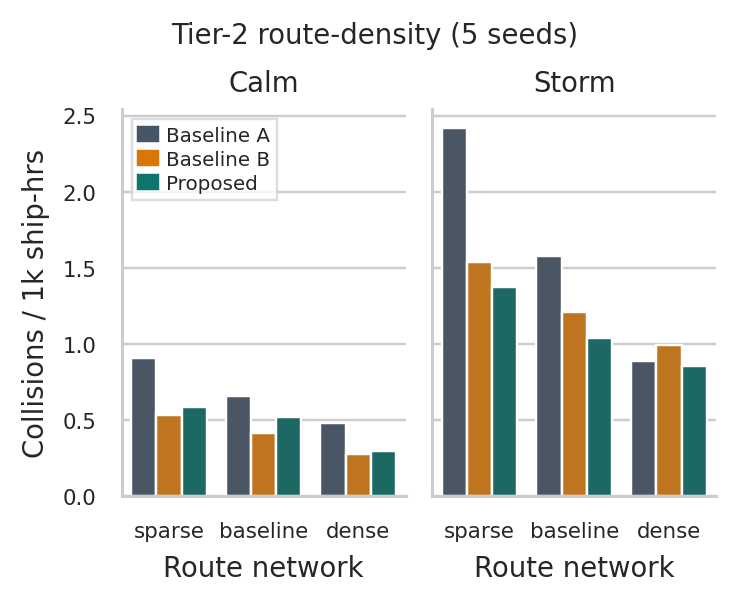
\includegraphics[width=\columnwidth]{figures/route_density.png}
\caption{Tier-2 collisions by route network, method, and scenario (five seeds).}
\label{fig:route-density}
\end{figure}

% ==================================================================
\section{Discussion}
\label{sec:discussion}
% ==================================================================

The core claim is Eq.~\ref{eq:pcomms}: a warning succeeds only when weather and both crews allow it. Across the definitive factorial (underway fleets, $\Delta t=5$\,min, stressor-specific horizons), all three primary hypotheses confirm: Blind Shore fatals (H1) and collisions (H3), and $P_{\mathrm{prep}}$ versus Baseline~A in every scenario (H2). Storm/Calm collision contrast is $3.71\times$ under Baseline~A. IWRAP stamps ($1.6$--$6.6$/yr for the multi-corridor domain) scale with fleet and method speed. Modelling limits that bound these claims are collected in Section~\ref{sec:limitations}.

% ==================================================================
\section{Limitations}
\label{sec:limitations}
% ==================================================================

The results should be read as evidence about the coupled weather--fatigue warning mechanism under a controlled Baltic--North Sea ABM, not as a census forecast of real casualties.

\begin{description}

  \item[Homogeneous crews and ships.]
  Every vessel carries the same crew count $n=20$. Manning in reality varies by flag, ship type, and voyage (IMO A.1047 leaves minima to Administrations~\cite{imo1047}); passenger ``hotel'' complements and fishing crews are omitted. Fatigue is a single scalar $F_i$ per ship with a shared circadian drive---not watch bills, individual seafarer states, or STCW rest-hour compliance. Vessel kinematics use class drafts for routing but share one contact radius, CPA gate, and give-way geometry; tankers, Ro-Pax, and feeders are not distinguished in manoeuvre latency or turning circles.

  \item[Time step and scenario horizons.]
  The engine advances at $\Delta t = 5$\,min so a typical bridge CPA/TCPA alarm band ($12$--$15$\,min) spans several ticks. Horizons are stressor-specific: Calm Passage is a $14$-day \emph{exposure} arm (not a claim of fortnight-long meteorological calm); Storm Corridor is an ${\approx}4$-day event with a translating cell crossing the domain in ${\approx}3$ days; Blind Shore and Deep Water Rescue run $7$ days. Baltic extreme-wave and surge events typically last hours to a few days, so month-long unbroken calm or basin-wide storm is deliberately avoided.

  \item[Traffic representation.]
  Routes are synthesised from bathymetry and AIS density (Section~\ref{sec:routegen}), not replayed voyages. Concurrent fleets ($N\in\{500,750,900\}$) target underway AIS scale~\cite{huetten2025baltic} while omitting stationary/moored traffic and North Sea inflation beyond the domain. Encounters use pairwise CPA with a lower-id give-way surrogate instead of full COLREGs hierarchy, multi-ship arbitration, or VTS intervention. Optional force-field avoidance stays off in definitive runs~\cite{xiao2013}. Port dwell is a uniform tick draw; cargo operations, pilotage, and anchorage queues are absent.

  \item[Consequence, SAR, and external checks.]
  SIMCOL damage and the SOLAS-shaped survival factor $S_i$ are surrogates, not residual-stability or finite-element hull models~\cite{lutzen2001,solas2020}. KPI fatalities count unrecovered persons-in-water only; liferaft \textsc{Lost} is logged separately and does not enter H1. SAR uses MASSIM/Koopman detection and Ashrafi seasonal factors without live RCC coordination or asset contention beyond the modelled helicopter/patrol pair~\cite{karatas2018,ashrafi2024}. IWRAP $N_c$ stamps use static network geometry and scenario fleet size, not per-run AIS tracks~\cite{friishansen2008iwrap}.

  \item[Statistics and scope.]
  Primary hypotheses are scoped to Blind Shore outcomes (H1, H3) and preparedness (H2) because patchy shore radio leaves room for the fatigue lever, whereas Storm Corridor shares an environmental blackout across methods. Holm correction is applied to that six-contrast primary battery; the full factorial heatmap is exploratory. Findings are specific to the Baltic--North Sea bbox, the three method configurations, and the chosen seeds; they do not transfer automatically to other basins, autonomous vessels, or adversarial AIS behaviour.

\end{description}

% ==================================================================
\section{Conclusions}
\label{sec:conclusions}
% ==================================================================

Section~\ref{sec:goal} asked whether linking fatigue management to warning reliability improves coordination and safety relative to classical practice. Under the definitive $360$-run design, the answer on the primary battery is \emph{yes}.

\begin{description}
  \item[H1] (Blind Shore: ${\geq}20\,\%$ fatal-rate cut vs Baseline~A) is \textbf{confirmed} ($0.486\to0.304$, ${\approx}37\,\%$, $\delta=0.53$).

  \item[H2] (Proposed raises $P_{\mathrm{prep}}$ vs Baseline~A in every scenario) is \textbf{confirmed} in all four settings ($|\delta|\in[0.52,1.00]$).

  \item[H3] (Blind Shore: ${\geq}10\,\%$ collision-rate cut vs Baseline~A) is \textbf{confirmed} ($1.26\to1.11$, ${\approx}12\,\%$, $\delta=0.54$).
\end{description}

Coupling weather and fatigue into $P_{\text{comms}}$ (Eq.~\ref{eq:pcomms}) therefore both raises preparedness and, under shore-comms stress, converts that lever into fewer collisions and fewer unrecovered MOB fatalities. Storm Corridor remains a hard environment for fatal method separation because environmental radio blackout is shared; Deep Water survival complements move directionally but are not primary claims. Future work should stress multi-ship COLREGs arbitration and heterogeneous manning.

\bibliographystyle{IEEEtran}
\bibliography{mybib}

% ==================================================================
\appendix
% ==================================================================

\section{Engine Internals}
\label{apx:engine}

This appendix mirrors the walkthrough style of an earlier coastal Mesa prototype, but every step and type name is taken from the current Rust engine in \texttt{crates/simulation} (\texttt{SimState::run\_tick}~/~\texttt{post\_tick}, \texttt{VesselAgent}, \texttt{WeatherField}, \texttt{sar}). Macro tick $\Delta t=5$\,min.

\subsection{SAR Asset State Machine}
\label{apx:sar-fsm}

Fig.~\ref{fig:sar-fsm} complements the vessel FSM of Fig.~\ref{fig:fsm}: once a founder enters \textsc{Evac}, a \texttt{RescueAgent} is dispatched from the nearest shore base (Helicopter beyond the open-water threshold, else Patrol). Speeds and boarding rates use Ashrafi month factors; on-scene detection uses Koopman CDP (Eq.~\ref{eq:cdp}). \texttt{MobSearchAgent} reuses the same \texttt{RescuePhase} enum but never enters Embarking---persons are recovered one-by-one while Searching.

\begin{figure}[t]
\centering
\resizebox{0.88\columnwidth}{!}{%
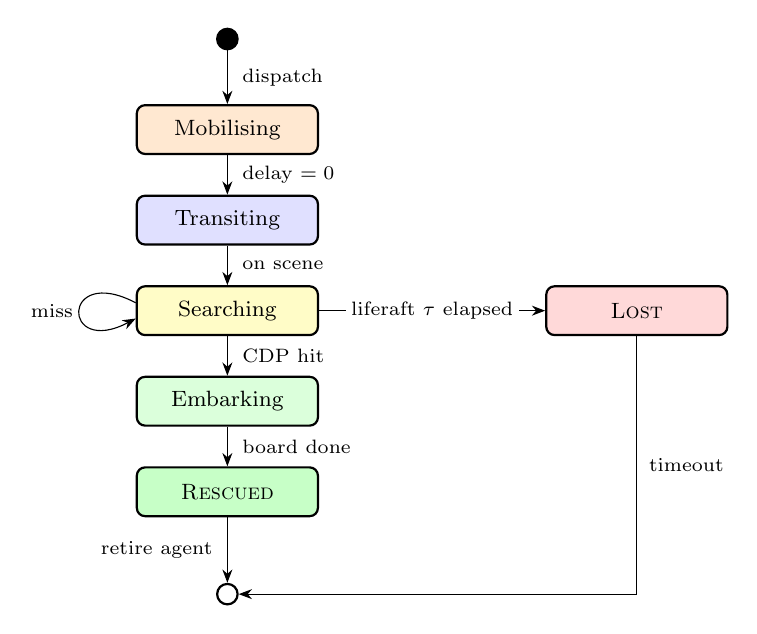
\begin{tikzpicture}[
  >=Stealth, font=\footnotesize,
  st/.style={draw, thick, rounded corners=3pt, minimum width=2.3cm,
             minimum height=0.62cm, align=center, inner sep=3pt},
  elab/.style={font=\scriptsize, inner sep=1.2pt, fill=white},
  term/.style={draw, thick, circle, minimum size=0.26cm, inner sep=0pt},
]
  \node[term, fill=black] (start) at (0,0) {};
  \node[st, fill=orange!18] (mob) at (0,-1.15) {Mobilising};
  \node[st, fill=blue!12] (tr) at (0,-2.3) {Transiting};
  \node[st, fill=yellow!22] (se) at (0,-3.45) {Searching};
  \node[st, fill=green!14] (em) at (0,-4.6) {Embarking};
  \node[st, fill=green!22] (ok) at (0,-5.75) {\textsc{Rescued}};
  \node[term, fill=white] (end) at (0,-7.05) {};

  \node[st, fill=red!15] (lost) at (5.2,-3.45) {\textsc{Lost}};

  \draw[->] (start) -- (mob) node[elab, midway, right=4pt]{dispatch};
  \draw[->] (mob) -- (tr) node[elab, midway, right=4pt]{delay $=0$};
  \draw[->] (tr) -- (se) node[elab, midway, right=4pt]{on scene};
  \draw[->] (se) -- (em) node[elab, midway, right=4pt]{CDP hit};
  \draw[->] (em) -- (ok) node[elab, midway, right=4pt]{board done};
  \draw[->] (ok) -- (end) node[elab, midway, left=4pt]{retire agent};

  \draw[->] ([yshift=1mm]se.west) .. controls +(-0.95,0.5) and +(-0.95,-0.5) ..
    node[elab, left=1pt]{miss} ([yshift=-1mm]se.west);

  \draw[->] (se.east) -- (lost.west)
    node[elab, midway, fill=white, inner sep=2pt]{liferaft $\tau$ elapsed};
  \draw[->] (lost.south) -- node[elab, right=3pt]{timeout}
    (lost.south |- end.east) -- (end.east);
\end{tikzpicture}%
}

\vspace{0.4em}
{\scriptsize
\textbf{MOB:} Mobilising$\to$Transiting$\to$Searching only (no Embarking);
each PIW draws CDP independently; agent retires when empty.}

\caption{UML state machine for \texttt{RescuePhase} on a liferaft \texttt{RescueAgent}. Vessel outcomes \textsc{Rescued}/\textsc{Lost} match Fig.~\ref{fig:fsm}; the asset is removed from \texttt{rescue\_agents} when the case closes.}
\label{fig:sar-fsm}
\end{figure}

\subsection{Macro-Tick Execution Sequence}
\label{apx:tick}

Table~\ref{tab:tick-steps} lists every step in source order. Step~1 is vessel navigation (krABMaga schedule order~$200$, or the inline loop in \texttt{run\_tick}); steps~2--13 are the shared \texttt{post\_tick} body invoked by \texttt{PostTickAgent} (order~$1000$) or by \texttt{run\_tick} after navigation, so the two paths cannot drift.

\begin{table*}[t]
\caption{Complete macro-tick execution sequence (\texttt{SimState}).}
\label{tab:tick-steps}
\centering
\small
\begin{tabularx}{\textwidth}{@{}c l >{\raggedright\arraybackslash}X@{}}
\toprule
\# & Phase & Action \\
\midrule
1 & Navigate & \textsc{Docked}: count down port dwell. \textsc{Active}: advance along the AIS route or an avoidance waypoint (follow-speed cap from the previous tick; skip if anchored). \textsc{Evac}/\textsc{Rescued}/\textsc{Lost}: no navigation. \\[2pt]
2 & Weather & \texttt{WeatherField::update}: calm/storm regime switch, grid storm-cell lifecycle, AR(1) sea/vis/wind channels, coupling, $5$-point smooth, fuse hazard $W$. \\[2pt]
3 & Grounding & Non-docked vessels on the land mask snap back to \texttt{last\_valid\_position} (no automatic \textsc{Evac}). \\[2pt]
4 & Fatigue / speed & \texttt{tick\_fatigue} from local $W$ and UTC. Methods B/P lerp the just-moved step by $f_W=\max(0.30,1-0.45\,W)$. If \texttt{storm\_pos} is set, apply \texttt{storm\_speed\_factor} inside the scenario storm radius (distinct from weather-grid cells). \\[2pt]
5 & Comms log & Emit \texttt{ResumeRoute} when an avoidance waypoint queue empties. \\[2pt]
6 & Avoidance & If \texttt{forcefield.enabled}: Xiao-style repulsion + Nomoto yaw (\texttt{apply\_force\_field}). Else: pairwise CPA inside \texttt{collision\_warn\_radius\_nm}; lower vessel id is give-way; with probability $P_{\text{comms}}$ (Eq.~\ref{eq:pcomms}; storm rate inside \texttt{storm\_pos}) inject starboard waypoint $(L_f,L_o)$ and log Warning$\to$GivingWay$\to$MaintainingCourse. Then decrement avoidance cooldowns. \\[2pt]
7 & Following & \texttt{compute\_following}: same-destination queueing / keep-distance (caps apply on the next navigate). \\[2pt]
8 & Collision & Rising-edge contact at \texttt{collision\_trigger\_field}${}=2r$; skip pairs inside port exclusion. Classify geometry; \texttt{simcol::evaluate} each struck ship; founder $\to$ \textsc{Evac}, else overboard count $\to$ \texttt{spawn\_mob\_incident}. \\[2pt]
9 & SAR & \texttt{run\_sar}: liferaft drift; dispatch \texttt{RescueAgent} (Helicopter if datum $\ge$ helo threshold, else Patrol) from nearest shore base; advance Mobilising$\to$Transiting$\to$Searching$\to$Embarking with Ashrafi month factors and Koopman CDP; timeout $\to$ \textsc{Lost}. \\[2pt]
10 & MOB & \texttt{run\_mob\_sar}: advect \texttt{MobPerson}s; advance \texttt{MobSearchAgent}s; recover on CDP draw or fatality when $\tau_{\text{mob}}$ elapses. \\[2pt]
11 & Reap & Drop \textsc{Rescued}/\textsc{Lost} vessels; tally cumulative rescued/lost. \\[2pt]
12 & KPI / fleet & Record ship-hours, collisions, fatals, $P_{\text{prep}}$; \texttt{spawn\_vessel} until $|\text{fleet}|=N$. \\[2pt]
13 & Housekeeping & Advance \texttt{utc\_hour} by $\Delta t$; \texttt{advance\_storm} along the scenario track; optional WebSocket snapshot / JSONL line. Macro \texttt{step} is incremented by \texttt{run\_tick} or set by krABMaga \texttt{State::update}, not inside \texttt{post\_tick}. \\
\bottomrule
\end{tabularx}
\end{table*}

\subsection{CPA Comms Sequence}
\label{apx:cpa-seq}

Fig.~\ref{fig:cpa-seq} expands Table~\ref{tab:tick-steps} step~6 for the default CPA track (force-field off). The lower vessel id is give-way; the higher id is stand-on. A uniform draw below $P_{\text{comms}}$ (Eq.~\ref{eq:pcomms}) commits the three-message exchange and injects the starboard waypoint; otherwise the pair is left to geometry until a later tick or hard contact (Fig.~\ref{fig:seq}).

\begin{figure*}[t]
\centering
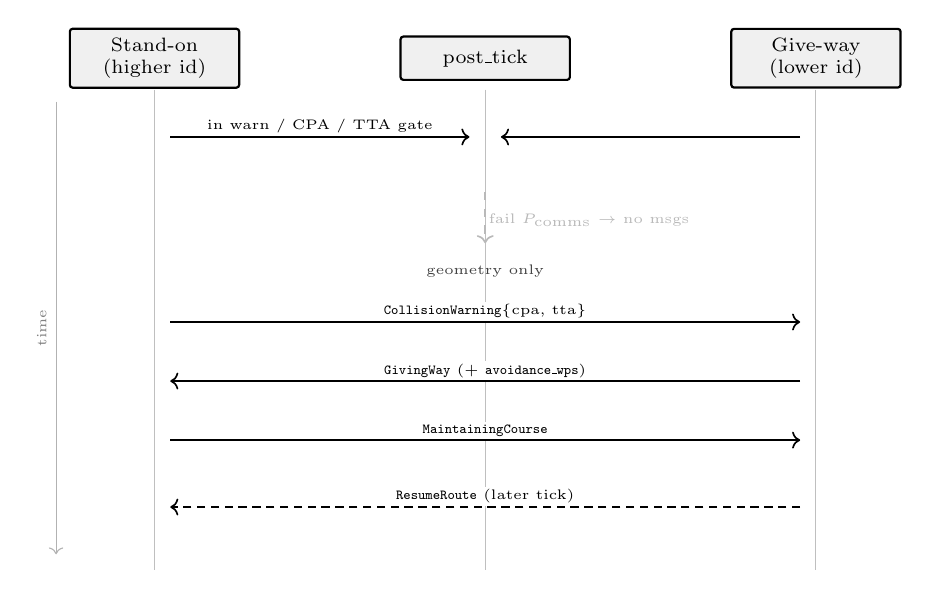
\begin{tikzpicture}[
  font=\scriptsize,
  actor/.style={draw, thick, minimum width=2.15cm, minimum height=0.55cm,
    align=center, fill=gray!12, rounded corners=1pt},
  msg/.style={->, semithick},
  nm/.style={font=\tiny, fill=white, inner sep=1pt},
]
  \node[actor] (so) at (0,0) {Stand-on\\(higher id)};
  \node[actor] (pt) at (4.2,0) {post\_tick};
  \node[actor] (gw) at (8.4,0) {Give-way\\(lower id)};

  \foreach \x in {0, 4.2, 8.4} {
    \draw[gray!50] (\x,-0.4) -- (\x,-6.5);
  }

  \draw[msg] (0.2,-1.0) -- (4.0,-1.0)
    node[nm, above, midway]{in warn / CPA / TTA gate};
  \draw[msg] (8.2,-1.0) -- (4.4,-1.0);

  \draw[msg, dashed, gray!55] (4.2,-1.7) -- (4.2,-2.35)
    node[nm, right, pos=0.55]{fail $P_{\text{comms}}$ $\to$ no msgs};
  \node[font=\tiny, text=gray!50!black] at (4.2,-2.7) {geometry only};

  \draw[msg] (0.2,-3.35) -- (8.2,-3.35)
    node[nm, above, midway]{\texttt{CollisionWarning}\{cpa, tta\}};
  \draw[msg] (8.2,-4.1) -- (0.2,-4.1)
    node[nm, above, midway]{\texttt{GivingWay} (+ \texttt{avoidance\_wps})};
  \draw[msg] (0.2,-4.85) -- (8.2,-4.85)
    node[nm, above, midway]{\texttt{MaintainingCourse}};
  \draw[msg, densely dashed] (8.2,-5.7) -- (0.2,-5.7)
    node[nm, above, midway]{\texttt{ResumeRoute} (later tick)};

  \draw[->, gray!60, thin] (-1.25,-0.55) -- (-1.25,-6.3)
    node[midway, left, font=\tiny, gray, rotate=90, anchor=south]{time};
\end{tikzpicture}
\caption{UML sequence for a successful CPA conversation (\texttt{MsgKind} in \texttt{comms.rs}). Failed $P_{\text{comms}}$ draws omit all three messages and the waypoint. \texttt{ResumeRoute} is logged when the give-way ship finishes the avoidance queue (Table~\ref{tab:tick-steps}, step~5).}
\label{fig:cpa-seq}
\end{figure*}

\subsection{Collision and Rescue Sequence}
\label{apx:seq}

Fig.~\ref{fig:seq} shows the rising-edge collision path that feeds liferaft evacuation and person-in-water (MOB) search after the CPA attempt of Fig.~\ref{fig:cpa-seq}. CPA avoidance (Table~\ref{tab:tick-steps}, step~6) runs \emph{before} hard contact (step~8) inside the same \texttt{post\_tick}, but a newly injected avoidance waypoint is consumed only on the \emph{next} navigate; within-tick order remains navigate-then-physics.

\begin{figure*}[t]
\centering
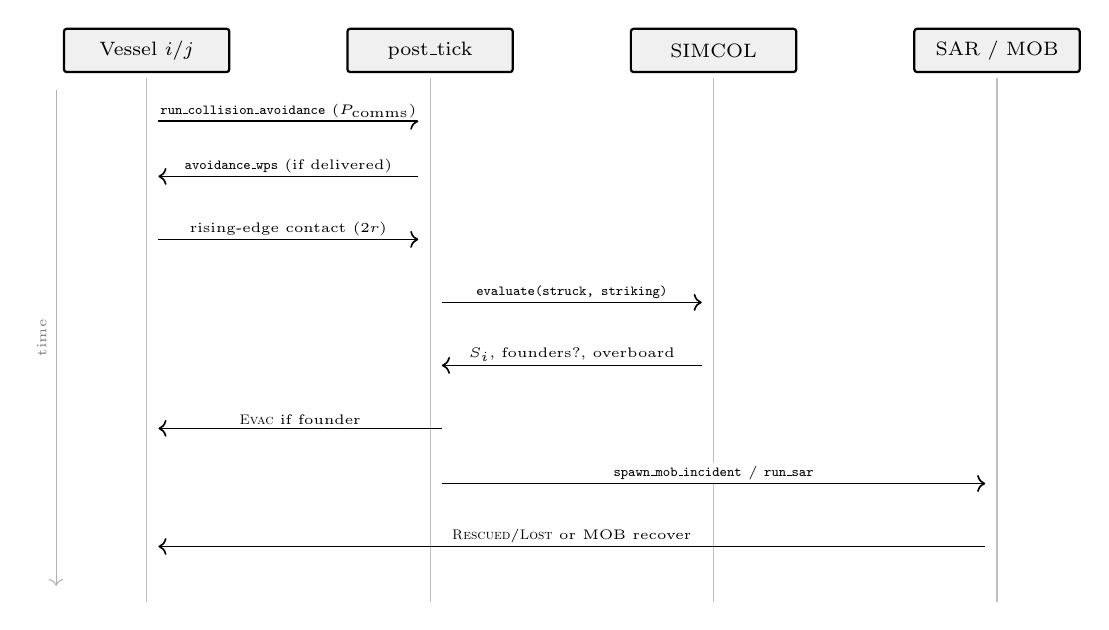
\begin{tikzpicture}[
  font=\scriptsize,
  actor/.style={draw, thick, minimum width=2.1cm, minimum height=0.55cm,
    align=center, fill=gray!12, rounded corners=1pt},
  msg/.style={->, semithick},
  nm/.style={font=\tiny, fill=white, inner sep=1pt},
]
  \node[actor] (v) at (0,0) {Vessel $i$/$j$};
  \node[actor] (pt) at (3.6,0) {post\_tick};
  \node[actor] (sc) at (7.2,0) {SIMCOL};
  \node[actor] (sar) at (10.8,0) {SAR / MOB};

  \foreach \x/\lab in {0/v, 3.6/pt, 7.2/sc, 10.8/sar} {
    \draw[gray!50] (\x,-0.35) -- (\x,-7.0);
  }

  \draw[msg] (0.15,-0.9) -- (3.45,-0.9)
    node[nm, above, midway]{\texttt{run\_collision\_avoidance} ($P_{\text{comms}}$)};
  \draw[msg] (3.45,-1.6) -- (0.15,-1.6)
    node[nm, above, midway]{\texttt{avoidance\_wps} (if delivered)};

  \draw[msg] (0.15,-2.4) -- (3.45,-2.4)
    node[nm, above, midway]{rising-edge contact ($2r$)};
  \draw[msg] (3.75,-3.2) -- (7.05,-3.2)
    node[nm, above, midway]{\texttt{evaluate(struck, striking)}};
  \draw[msg] (7.05,-4.0) -- (3.75,-4.0)
    node[nm, above, midway]{$S_i$, founders?, overboard};

  \draw[msg] (3.75,-4.8) -- (0.15,-4.8)
    node[nm, above, midway]{\textsc{Evac} if founder};
  \draw[msg] (3.75,-5.5) -- (10.65,-5.5)
    node[nm, above, midway]{\texttt{spawn\_mob\_incident} / \texttt{run\_sar}};
  \draw[msg] (10.65,-6.3) -- (0.15,-6.3)
    node[nm, above, midway]{\textsc{Rescued}/\textsc{Lost} or MOB recover};

  \draw[->, gray!60, thin] (-1.15,-0.5) -- (-1.15,-6.8)
    node[midway, left, font=\tiny, gray, rotate=90, anchor=south]{time};
\end{tikzpicture}
\caption{UML sequence aligned with \texttt{post\_tick}: CPA (or force-field) first, then hard contact, SIMCOL, \texttt{run\_sar} / \texttt{run\_mob\_sar}. Survival windows are liferaft ticks for \textsc{Evac} and $\tau_{\text{mob}}$ for persons in the water. Asset phases appear in Fig.~\ref{fig:sar-fsm}.}
\label{fig:seq}
\end{figure*}

\section{Default Constants}
\label{apx:constants}

Table~\ref{tab:constants} lists principal defaults (overridable in configuration). Scenario overrides that differ from these defaults appear in Table~\ref{tab:scenarios}.

\begin{table*}[t]
    \caption{Selected engine default constants (role and value rationale). Scenario overrides appear in Table~\ref{tab:scenarios}; longer discussion in Section~\ref{sec:param-rationale}.}
    \label{tab:constants}
    \centering
    \footnotesize
    \setlength{\tabcolsep}{3.5pt}
    \begin{tabular}{@{}llp{1\columnwidth}@{}}
        \toprule
        Constant & Default & Role / rationale \\
        \midrule
        $\Delta t$, $T$ & $5$\,min; $14$/$4$/$7$\,d &
        Tick; Calm / Storm / Blind·Deep horizons (exposure vs event) \\
        $N$ vessels & $750$ &
        Concurrent \emph{underway} agents: Baltic AIS mean ${\approx}774$ moving ships~\cite{huetten2025baltic} (HELCOM ${\approx}2000$ total at sea~\cite{helcom2010}); Storm/Blind $900$, Deep Water $500$. Stationary/moored omitted. \\
        $n$ crew & $20$ &
        Fleet-mean overboard exposure; IMO A.1047 leaves manning to Administrations~\cite{imo1047}; cargo/tanker practice ${\approx}15$--$25$~\cite{helcom2010}. \\
        weather grid; $(w_s,w_v,w_u)$ & $50\times50$; $(1.0,0.5,0.8)$ &
        Spatially resolved hazard for $W$; sea-state weighted highest as the dominant radio/perception stressor. \\
        $q$ (nominal link) & $1.0$ &
        Perfect fair-weather VHF/AIS baseline so Blind Shore ($0.55$) and storm-comms isolate degradation. \\
        warn / CPA / TTA gate & $25$ / $8$\,nm / $48$ tk &
        Early COLREGs-style detection (${\approx}4$\,h); wider CPA berth at concurrent density~\cite{colregs1972,tam2010}. \\
        $L_f,L_o$; cooldown & $5$ / $9$\,nm; $2$ tk &
        Larger starboard give-way offset (Eq.~\ref{eq:avoidwp}); ${\approx}10$\,min lockout at $\Delta t=5$\,min. \\
        waypoint reach & $0.5$\,nm &
        Capture radius ${\approx}$ ship-length scale so pursuit does not chatter at each vertex. \\
        $r_{\text{coll}}$; port exclusion & $0.012$\,nm; $2.5$\,nm &
        Hard hit at $2r{=}0.024$\,nm (${\approx}45$\,m, beam-scale) so Calm A stays in $0.5$--$2.0$/\,1k ship-hrs at $\Delta t=5$\,min; harbour water excluded. \\
        follow vicinity / gap; same-dest. & $3$ / $0.5$\,nm; $5$\,nm &
        Queueing on shared lanes: speed-match and hold-station without side-by-side overlap the give-way rule misses. \\
        dwell & $24$--$144$ tk &
        Uniform $2$--$12$\,h port stay spreads departures and avoids convoy synchrony. \\
        $m(\text{A/B/Proposed})$ & $1.00/0.82/0.65$ &
        Method lever on Eq.~\ref{eq:m}: unmanaged / shore-rest / smart watch (H1--H3 ordering). \\
        $(\beta_{\text{base}},\beta_W,\beta_c)$ & $0.0005,0.00133,0.000267$ &
        Per $5$\,min tick (scaled from a $15$\,min calibration so hourly build is unchanged)~\cite{chauvin2013}. \\
        recovery; $F^\ast,\kappa$ & ${\approx}0.0083$/tk; $0.40,0.65$ &
        Dock rest clears fatigue in ${\approx}10$\,h; knee/penalty shape $g(F)$ so only elevated $F$ cuts $P_{\text{comms}}$. \\
        $\alpha_M$; fatigue weight & $2.0/1.3/1.0$; $0.70$ &
        Awareness weights for $P_{\text{prep}}$ (A most weather-sensitive); $0.70$ keeps fatigue material beside $W$. \\
        $f_W$ (B, Proposed) & $\max(0.30,\,1-0.45\,W)$ &
        Weather-aware slowdown floor $0.30$; Baseline~A ignores (no mitigation). \\
        storm radius / drift & $120$\,nm / ${\approx}1.0$\,nm/tk &
        Corridor: $160$\,nm cell at ${\approx}12$\,kn (${\approx}3$\,d Channel$\to$Gda\'nsk). \\
        storm-comms & $0.30$ ($0.08$ Corridor) &
        Environmental blackout shared by all methods; Corridor near-blackout (exploratory vs Blind H1/H3). \\
        storm speed factor & $0.70$ &
        Weather-aware crawl; A stays $1.0$; Corridor non-A $0.45$ for stronger Storm/Calm contrast. \\
        force-field track & off &
        Optional Xiao-style repulsion~\cite{xiao2013}; off keeps discrete give-way as the primary COLREGs path. \\
        $(m_{\text{sway}},m_{\text{surge}})$ & $0.85,0.05$ &
        DTU SIMCOL added-mass defaults~\cite{lutzen2001}. \\
        Minorsky $a,b$ & $47.2,32.7$ &
        Classical energy--volume coefficients (MJ, m$^3$)~\cite{minorsky1959}. \\
        $\ell/L_{pp},\tau$ & $0.12$, $0.08$\,m &
        Damage-length fraction and side-shell thickness in the SIMCOL penetration surrogate. \\
        $r_0,r_1,S^{\dagger}$ & $0.10,0.30,0.35$ &
        SOLAS-shaped $S_i$ knees~\cite{solas2020}; $S^{\dagger}{=}0.35$ keeps moderate damage afloat $\to$ MOB path (\texttt{fatal\_per\_1k\_hrs}). \\
        helo / patrol; cutoff & $80$ / $25$\,kn; $40$\,nm &
        Typical SAR asset speeds; $40$\,nm selection range (Deep Water slows assets; Section~\ref{sec:param-rationale}). \\
        $\Delta t_{\text{mob}}$; arrival $r$ & $6$ tk; $1$\,nm &
        $30$\,min readiness (${\approx}1$\,h Deep); datum capture radius before search starts. \\
        $w,\,r_0^{\text{SAR}},\,u_d$ & $5$, $2$\,nm, ${\approx}0.067$\,nm/tk &
        MASSIM/Koopman sweep width, initial search radius, and ${\approx}0.8$\,kn drift~\cite{karatas2018,koopman1980}. \\
        survival / $\tau_{\text{mob}}$ & $288$ / $18$ tk &
        Liferaft $24$\,h; MOB ${\approx}1.5$\,h in colder IAMSAR immersion bands~\cite{imosar2018,tipton2022survival}. \\
        MOB scatter; searchers & $0.5$\,nm; $1$ &
        Compact person-in-water cloud; one search team keeps rescue latency on the critical path. \\
        sim.\ month & July (Ashrafi A); Deep Water Jan (D) &
        Mild default vs winter Group~D degradation (exploratory Deep arm)~\cite{ashrafi2024}. \\
        $P_c$ (IWRAP) & $0.5$--$1.3{\times}10^{-4}$ &
        IALA IWRAP Mk~II causation defaults (head-on / overtaking / crossing)~\cite{friishansen2008iwrap}. \\
        route weights $(w_h,w_d,w_\ell)$ & $(3,4,2.5)$ &
        Offline A\textsuperscript{*} prefers depth and lane density over raw length (Section~\ref{sec:routegen}). \\
        UKC buffer $m_s$ & $2$\,m &
        Extra navigable margin beyond charted UKC for offline bathymetry routing. \\
        draft+UKC (pax/cargo/tanker) & $6.5{+}1.5$ / $11{+}2$ / $14{+}3$\,m &
        Baltic--North Sea class drafts: Ro-Pax ${\approx}6.4$\,m~\cite{gucma2018ropax}; cargo/tanker under PIANC~\cite{pianc2014}. \\
        \bottomrule
    \end{tabular}
\end{table*}

Weather-field process (Mixed preset): regime flips $p_{cs}=0.01$, $p_{sc}=0.027$ per $5$\,min tick; Calm/Storm reversion targets $(0.30,0.80,0.25)$ / $(0.72,0.30,0.75)$; up to $8$ storm cells; AR(1) coefficients $(\rho_s,\rho_v,\rho_u)\approx(0.983,0.965,0.976)$, $(\sigma_s,\sigma_v,\sigma_u)=(0.07,0.06,0.07)$; gradient cap $0.12$. Calm and Stormy presets scale the flip rates.

\section{Playback Workbench}
\label{apx:gui}

The optional React~19 / Vite workbench is a batch-first client for the Axum API: it does not run the ABM in the browser. Figure~\ref{fig:gui-overview} shows the shell---a permanent left panel beside a full-bleed deck.gl map over a MapLibre basemap. Under \textsc{Runs}, the operator selects scenarios and methods, seed/tick counts, and an optional JSON config override, then posts a factorial batch; progress arrives over SSE while finished seeds appear in a completed-run list. Selecting a seed loads its JSONL tick log and enables the pinned playback dock (play/pause, speed, scrubber). Map layers render vessels and ports, AIS route context, weather/storm overlays, collisions and wrecks, and SAR/MOB entities, with camera and layer toggles in the map chrome.

\begin{figure*}[t]
\centering
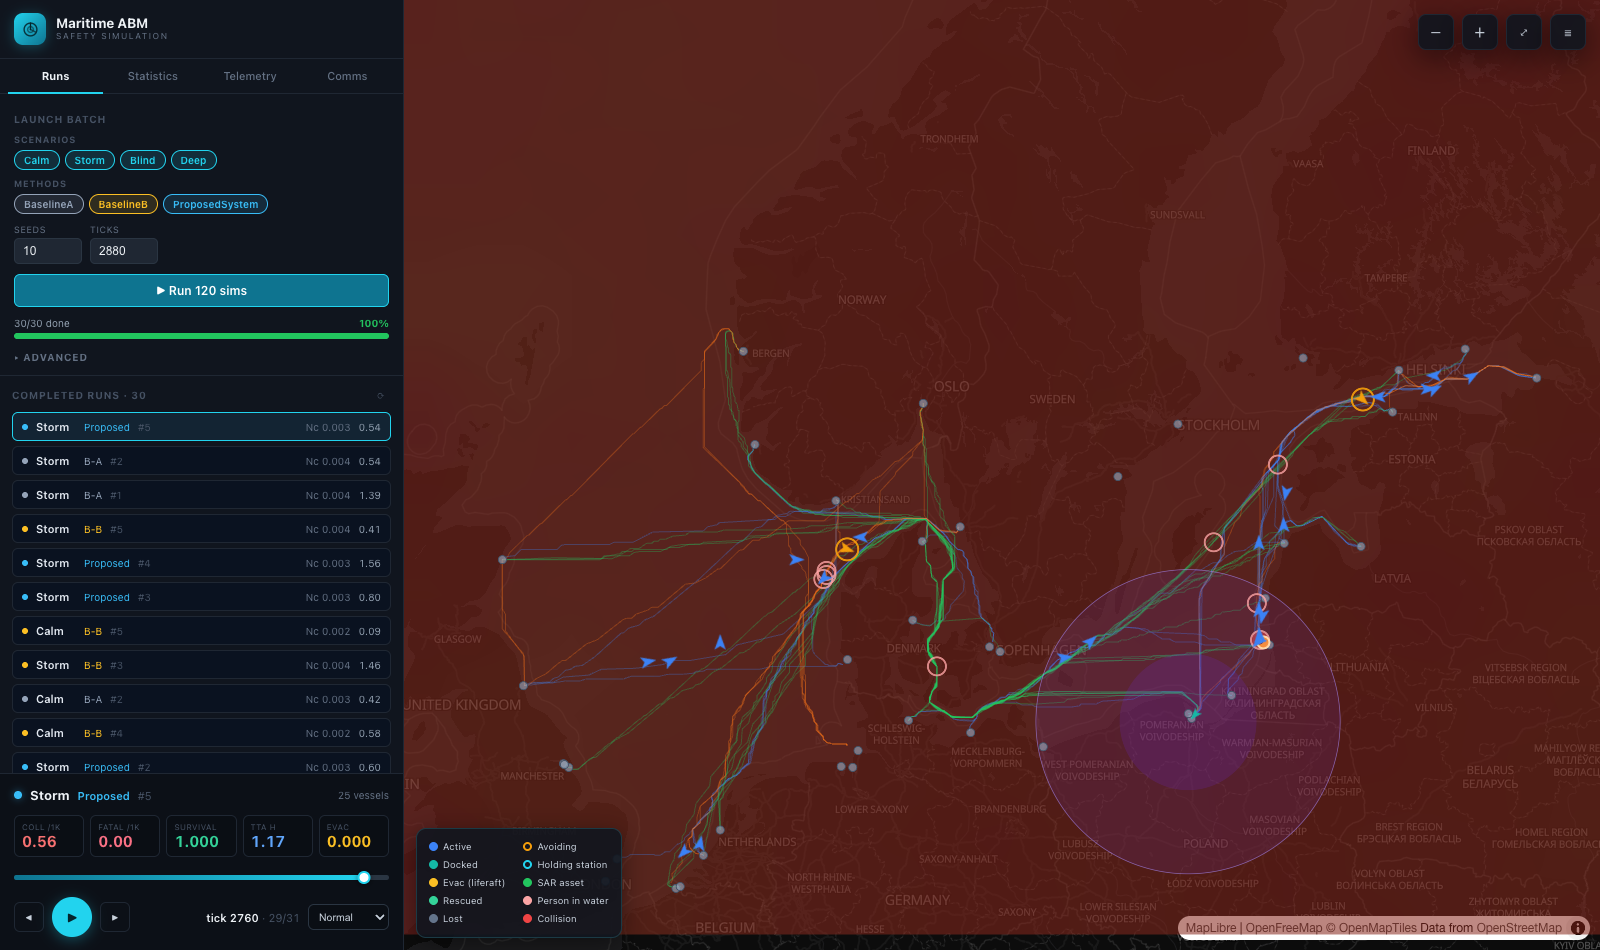
\includegraphics[width=\textwidth]{figures/gui_overview.png}
\caption{Workbench shell scrubbed mid-run (Storm Corridor, Proposed, seed~5, tick~$2760$): live KPI tiles, vessel tracks / avoidance rings / collisions on the map, and the storm disc over the southern Baltic.}
\label{fig:gui-overview}
\end{figure*}

Figure~\ref{fig:gui-comms} shows the \textsc{Comms} tab: bridge messages up to the scrubber (collision warnings with CPA/TTA, give-way, resume-route, keep-distance). \textsc{Statistics} and \textsc{Telemetry} (not shown) pull pairwise Mann--Whitney / Holm summaries and KPI time series for the active batch. The GUI is for inspection and debugging---all hypothesis numbers in the main text come from exported batch JSON / SQLite, not from the browser.

\begin{figure*}[t]
\centering
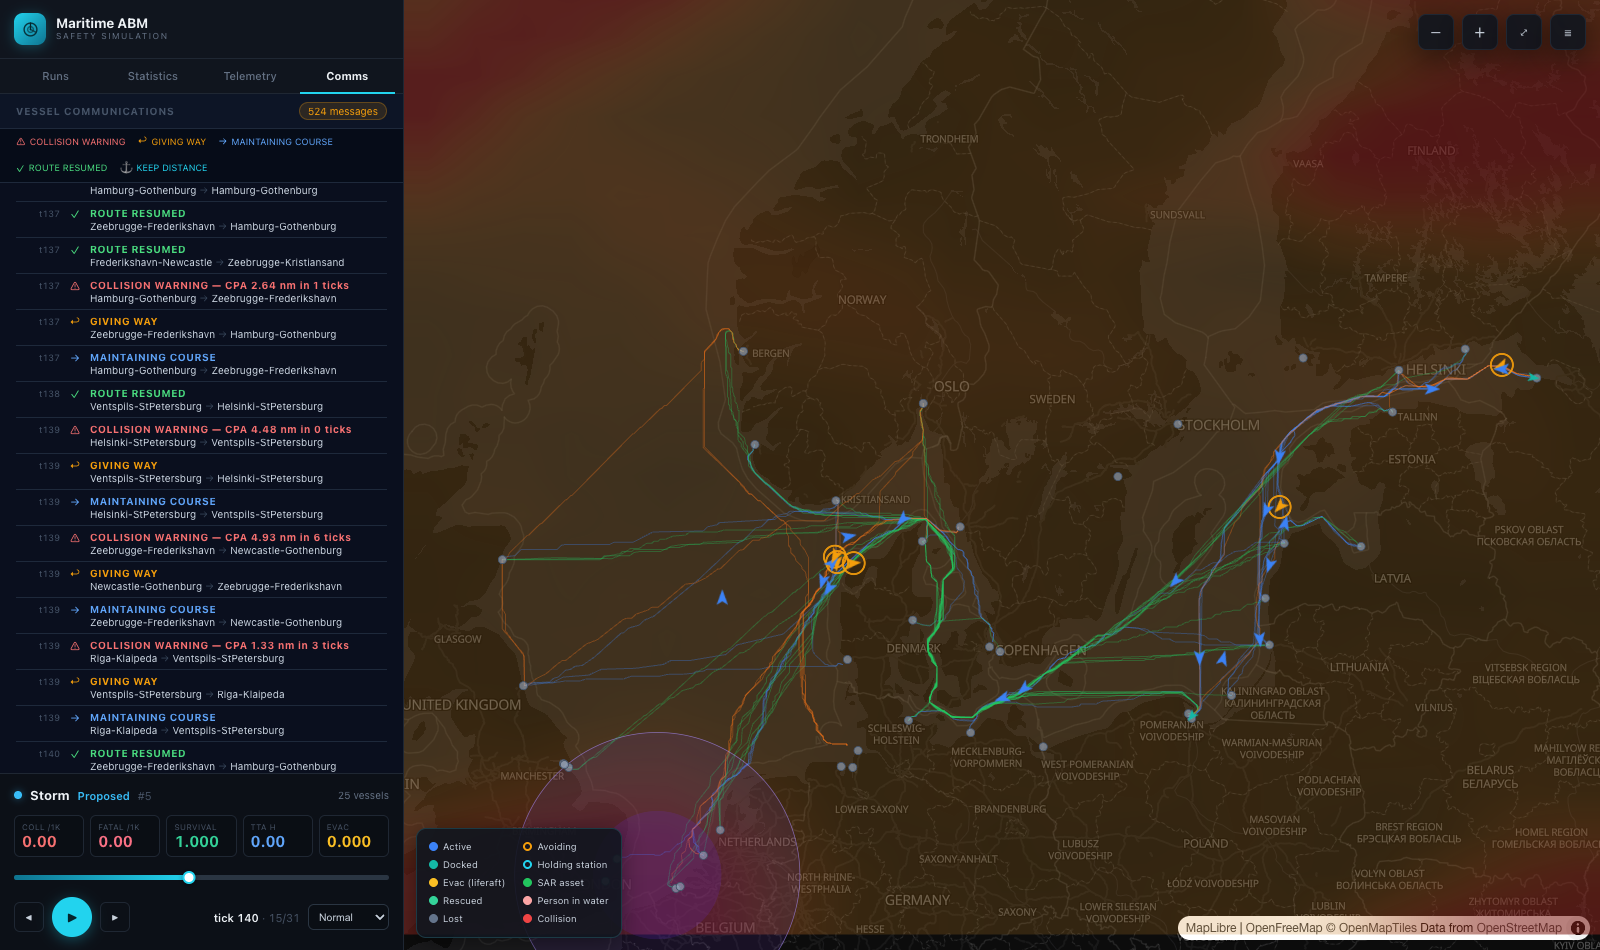
\includegraphics[width=\textwidth]{figures/gui_comms.png}
\caption{Comms log for the same Storm Corridor run (hundreds of VHF-style messages with CPA warnings and give-way acknowledgements), with the playback map still showing routes and the moving storm.}
\label{fig:gui-comms}
\end{figure*}

\end{document}
